%                                                                 aa.dem
% AA vers. 8.2, LaTeX class for Astronomy & Astrophysics
% demonstration file
%                                                       (c) EDP Sciences
%-----------------------------------------------------------------------
%
%\documentclass[referee]{aa} % for a referee version
%\documentclass[onecolumn]{aa} % for a paper on 1 column  
%\documentclass[longauth]{aa} % for the long lists of affiliations 
%\documentclass[rnote]{aa} % for the research notes
%\documentclass[letter]{aa} % for the letters 
%\documentclass[bibyear]{aa} % if the references are not structured 
% according to the author-year natbib style

%%%%%%%%%%%%%%%%%%%%%%%%%%%%%%%%%%%%%%%%%%%%%%%%%%%%%%%%%%%%%%%%%%%%%%%%%%%%
\documentclass{aa}    %% Astronomy & Astrophysics style class aa.cls v8.2
%\documentclass[referee]{aa} 

\usepackage{graphicx,url,twoopt,natbib}
\usepackage[varg]{txfonts}           %% A&A font choice

\usepackage{pdfcomment}              %% for popup acronym meanings
\usepackage{acronym}                 %% for popup acronym meanings

\usepackage{url}
\usepackage{color,hyperref}
\definecolor{linkcolor}{rgb}{0,0.3,0.7}
\hypersetup{colorlinks=true,
	linkcolor=linkcolor, 
	citecolor=linkcolor,
	filecolor=linkcolor, 
	urlcolor=linkcolor}

\usepackage{natbib}
\usepackage{caption}

\bibpunct{(}{)}{;}{a}{}{,}    %% natbib cite format used by A&A and ApJ

% Manually specified definitions
\newcommand{\farc}{\hbox{$.\!\!^{\prime\prime}$}} 
\newcommand{\ergA}{$\rm{erg\,cm^{-2}\,s^{-1}\,\AA^{-1}}$} 
\newcommand{\erg}{$\rm{erg\,cm^{-2}\,s^{-1}}$} 
\newcommand{\kms}{$\rm{km\,s^{-1}}\,$}

\newcommand{\griz}{$g' r' i' z'$}
\newcommand{\JHK}{$JHK_{\rm{s}}$}
\newcommand{\gK}{$g' r' i' z' JHK_{\rm{s}}$}
\newcommand{\Msun}{$M_\odot$}


% Elements
\newcommand{\lya}{Ly$\alpha$} 
\newcommand{\lyb}{Ly$\beta$} 
\newcommand{\lyg}{Ly$\gamma$} 
\newcommand{\hb}{H$\beta$} 
\newcommand{\ha}{H$\alpha$} 
\newcommand{\hg}{H$\gamma$} 
\newcommand{\hd}{H$\delta$} 
\newcommand{\pab}{Pa$\beta$} 
\newcommand{\paa}{Pa$\alpha$} 
\newcommand{\pag}{Pa$\gamma$} 
\newcommand{\pad}{Pa$\delta$} 



\newcommand{\cah}{Ca H} 
\newcommand{\cak}{Ca K} 
\newcommand{\cahk}{Ca H \& K} 
\newcommand{\nai}{Na ID} 


\newcommand{\hi}{\ion{H}{i}} 
\newcommand{\hei}{\ion{He}{i}} 
\newcommand{\oi}{\ion{O}{i}} 
\newcommand{\sii}{\ion{S}{ii}} 
\newcommand{\siii}{\ion{S}{iii}} 
\newcommand{\oii}{[\ion{O}{ii}]} 
\newcommand{\oiii}{[\ion{O}{iii}]}
\newcommand{\nii}{\ion{N}{ii}} 
\newcommand{\nv}{[\ion{N}{v}]} 
\newcommand{\neiii}{[\ion{Ne}{iii}]} 
\newcommand{\NIii}{\ion{Ni}{ii}} 
\newcommand{\feii}{\ion{Fe}{ii}} 
\newcommand{\civ}{\ion{C}{iv}} 
\newcommand{\cii}{\ion{C}{ii}}
\newcommand{\mgi}{\ion{Mg}{i}} 
\newcommand{\mgii}{\ion{Mg}{ii}} 
\newcommand{\ali}{\ion{Al}{i}} 
\newcommand{\alii}{\ion{Al}{ii}} 
\newcommand{\aliii}{\ion{Al}{iii}} 
\newcommand{\SIi}{\ion{Si}{i}} 
\newcommand{\SIii}{\ion{Si}{ii}} 
\newcommand{\SIiii}{\ion{Si}{iii}} 
\newcommand{\SIiv}{\ion{Si}{iv}} 
\newcommand{\znii}{\ion{Zn}{ii}} 
\newcommand{\crii}{\ion{Cr}{ii}} 
\newcommand{\mnii}{\ion{Mn}{ii}} 
\newcommand{\mni}{\ion{Mn}{i}} 
\newcommand{\tiii}{\ion{Ti}{ii}} 
\newcommand{\caii}{\ion{Ca}{ii}} 
\newcommand{\ariii}{\ion{Ar}{iii}} 
\newcommand{\TIii}{\ion{Ti}{ii}} 
\newcommand{\scii}{\ion{Sc}{ii}} 
%

\newcommand{\startdate}{$14/03/2009$} 
%\newcommand{\startdate}{14.03.2009} 

\newcommand{\termdate}{$31/03/2017$} 
%\newcommand{\termdate}{31.03.2017} 

\newcommand{\swift}{\textit{Swift}} 
\newcommand{\nhx}{$\log (N_{\mathrm{HI, X}}/\mathrm{cm}^{-2})$} 
\newcommand{\nh}{$\log (N_{\mathrm{HI}}/\mathrm{cm}^{-2})$} 


\usepackage{xcolor}
\newcommand\todo[1]{\textbf{(#1)}}

\begin{document}
	
\title{XSGRB - The X-shooter GRB afterglow sample
\thanks{Based on observations collected at the European Southern Observatory, Paranal, 
	Chile, Program ID: 098.A-0055, 097.A-0036, 096.A-0079, 095.B-0811(B), 
	095.A-0045, 094.A-0134, 093.A-0069, 092.A-0124, 0091.C-0934, 090.A-0088,
	089.A-0067, 088.A-0051, 087.A-0055, 086.A-0073, 085.A-0009 and 084.A-0260}}

\titlerunning{The X-shooter sample of GRBs}

\author{
J.~Selsing \inst{1, 2}$^,$\thanks{\email{jselsing@dark-cosmology.dk}}\addtocounter{footnote}{2}
\and D.~Malesani \inst{1, 2, 3}\fnmsep\thanks{On-call observer}
\and P.~Goldoni \inst{4, 7}\fnmsep$^\dagger$
\and J.~P.~U. Fynbo \inst{1, 2}\fnmsep$^\dagger$
\and T.~Kr\"{u}hler \inst{5}\fnmsep$^\dagger$
\and L.~A.~Antonelli \inst{6}\fnmsep$^\dagger$
\and M.~Arabsalmani \inst{7, 8}
\and J.~Bolmer \inst{5, 9}\fnmsep$^\dagger$
\and Z.~Cano \inst{10}\fnmsep$^\dagger$
\and L.~Christensen \inst{1}
\and S.~Covino \inst{11}\fnmsep$^\dagger$
\and P.~D'Avanzo \inst{11}\fnmsep$^\dagger$
\and V.~D'Elia \inst{12}\fnmsep$^\dagger$
\and A.~De~Cia \inst{13}
\and A.~de~Ugarte~Postigo \inst{1, 10}\fnmsep$^\dagger$
\and H.~Flores \inst{14}\fnmsep$^\dagger$
\and M.~Friis \inst{15, 16}
\and A.~Gomboc \inst{17}
\and J.~Greiner \inst{5}
\and P.~Groot \inst{18}
\and F.~Hammer \inst{14}
\and O.E.~Hartoog \inst{19}\fnmsep$^\dagger$
\and K.~E.~Heintz \inst{1, 2, 20}\fnmsep$^\dagger$
\and J.~Hjorth \inst{1}\fnmsep$^\dagger$
\and P.~Jakobsson \inst{20}\fnmsep$^\dagger$
\and J.~Japelj \inst{19}\fnmsep$^\dagger$
\and D.~A.~Kann \inst{10}\fnmsep$^\dagger$
\and L.~Kaper \inst{19}
\and C.~Ledoux \inst{9}
\and G.~Leloudas \inst{1}
\and A.J.~Levan \inst{21}\fnmsep$^\dagger$
\and E.~Maiorano \inst{22}
\and A.~Melandri \inst{11}\fnmsep$^\dagger$
\and B.~Milvang-Jensen \inst{1, 2}
\and E.~Palazzi \inst{22}
\and J.~T.~Palmerio \inst{23}\fnmsep$^\dagger$
\and D.~A.~Perley \inst{24}\fnmsep$^\dagger$
\and E.~Pian \inst{22}
\and S. ~Piranomonte \inst{6}\fnmsep$^\dagger$
\and G.~Pugliese \inst{19}\fnmsep$^\dagger$
\and R.~S\'{a}nchez-Ram\'{\i}rez \inst{25}\fnmsep$^\dagger$
\and S.~Savaglio \inst{26}
\and P.~Schady \inst{5}
\and S.~Schulze \inst{27}\fnmsep$^\dagger$
\and J.~Sollerman \inst{28}
\and M.~Sparre \inst{29}\fnmsep$^\dagger$
\and G.~Tagliaferri \inst{11}
\and N.~R.~Tanvir \inst{30}\fnmsep$^\dagger$
\and C.~C.~Th\"{o}ne \inst{10}
\and S.D.~Vergani \inst{14}\fnmsep$^\dagger$
\and P.~Vreeswijk \inst{18, 26}\fnmsep$^\dagger$
\and D.~Watson \inst{1, 2}\fnmsep$^\dagger$
\and K.~Wiersema \inst{21, 30}\fnmsep$^\dagger$
\and R.~Wijers \inst{19}
\and D.~Xu \inst{31}\fnmsep$^\dagger$
\and T.~Zafar \inst{32}
}
\institute{Dark Cosmology Centre, Niels Bohr Institute, University of Copenhagen, Juliane Maries Vej 30, 2100 K\o benhavn \O, Denmark %1
\and The Cosmic Dawn Center (DAWN), Niels Bohr Institute, University
of Copenhagen, Juliane Maries Vej 30, DK-2100 Copenhagen \O;
DTU-Space, Technical University of Denmark, Elektrovej 327,
DK-2800 Kgs.\ Lyngby
\and DTU Space, National Space Institute, Technical University of Denmark, Elektrovej 327, 2800 Lyngby, Denmark
\and APC, Astroparticule et Cosmologie, Universit\'e Paris Diderot, CNRS/IN2P3, CEA/Irfu, Observatoire de Paris, Sorbonne Paris Cit\'e, 10, Rue Alice Domon et L\'eonie Duquet, 75205, Paris Cedex 13, France
\and Max-Planck Institut f\"{u}r extraterrestrische Physik, Giessenbachstra\ss e 1, 85748 Garching, Germany
\and INAF - Osservatorio Astronomico di Roma, Via Frascati 33, 00078, Monte Porzio Catone (Roma), Italy
\and IRFU, CEA, Universit\'e Paris-Saclay, F-91191 Gif-sur-Yvette, France
\and Universit\'e Paris Diderot, AIM, Sorbonne Paris Cit\'e, CEA, CNRS, F-91191 Gif-sur-Yvette, France
\and European Southern Observatory, Alonso de C\'{o}rdova 3107, Vitacura, Casilla 19001, Santiago 19, Chile
\and Instituto de Astrof\'isica de Andaluc\'ia (IAA-CSIC), Glorieta de la Astronom\'ia s/n, E-18008, Granada, Spain. % 10
\and INAF - Osservatorio Astronomico di Brera, via Bianchi 46, 23807, Merate (LC), Italy
\and Space Science Data Center - Agenzia Spaziale Italiana, via del Politecnico, s.n.c., I-00133, Roma, Italy
\and European Southern Observatory, Karl-Schwarzschild Str. 2, 85748 Garching bei M\"unchen, Germany
\and GEPI, Observatoire de Paris, PSL University, CNRS, 5 place Jules Janssen 92195, Meudon, France
\and KTH Royal Institute of Technology, Department of Physics, 106 91 Stockholm, Sweden
\and The Oskar Klein Centre for Cosmoparticle Physics, AlbaNova University Centre, 106 91 Stockholm, Sweden
\and Center for Astrophysics and Cosmology, University of Nova Gorica, Vipavska 11c, 5270 Ajdov\v s\v cina, Slovenia
\and Department of Astrophysics, IMAPP, Radboud University Nijmegen, PO Box 9010, 6500 GL Nijmegen, the Netherlands
\and Anton Pannekoek Institute for Astronomy, University of Amsterdam, Science Park 904, 1098 XH Amsterdam, the Netherlands
\and Centre for Astrophysics and Cosmology, Science Institute, University of Iceland, Dunhagi 5, 107, Reykjavik, Iceland
\and Department of Physics, University of Warwick, Coventry, CV4 7AL, UK % 20
\and IASF/INAF Bologna, via Piero Gobetti 101, 40129 Bologna, Italy
\and Sorbonne Universit\'e, CNRS, UMR7095, Institut d'Astrophysique de Paris, F-75014, Paris, France
\and Astrophysics Research Institute, Liverpool John Moores University, IC2, Liverpool Science Park, 146 Brownlow Hill, Liverpool L3 5RF, UK
\and INAF, Istituto Astrofisica e Planetologia Spaziali, Via Fosso del Cavaliere 100, I-00133 Roma, Italy
\and Physics Department, University of Calabria, I-87036 Arcavacata di Rende, Italy
\and Department of Particle Physics and Astrophysics, Weizmann Institute of Science, 234 Herzl Street, Rehovot, 761000, Israel
\and Department of Astronomy, Stockholm University, AlbaNova, 10691 Stockholm, Sweden 
\and Institut f\"ur Physik und Astronomie, Universit\"at Potsdam, Karl-Liebknecht-Str.\,24/25, 14476 Golm, Germany
\and Department of Physics and Astronomy, University of Leicester, University Road, Leicester, LE1 7RH, United Kingdom
\and CAS Key Laboratory of Space Astronomy and Technology, National Astronomical Observatories, Chinese Academy of Sciences, Beijing, 100012, P.R. China % 30
\and Australian Astronomical Observatory, PO Box 915, North Ryde, NSW 1670, Australia.
}

\date{Received/ accepted}


\authorrunning{Selsing et al.}

\abstract{
In this work we present the spectra of \textit{all} $\gamma$-ray bursts (GRBs)
afterglows that have \textit{ever} been observed at the VLT/X-shooter up to the end of 2016. This
totals 137 spectroscopic observation of 118 individual bursts, of which
redshifts have been secured for 91 \% covering a redshift range from 0.059 to
$\sim$ 8.5. Based on a set of unbiasing selection criteria, the follow-up effort
has been guided by the \textit{Swift}-telescope to produce a homogeneous sample
of afterglows for 86 spectra, representing the underlying \textit{Swift} GRB population.
We here provide a public release of all the spectra, including continuum
estimates and telluric corrections. We provide an assessment of the degree of
completeness with respect to the parent GRB population, in terms of the X-ray
properties of the bursts in the sample and find that the sample presented here
can not be significantly distinguished from the \textit{Swift} sample.
For all bursts (39) for which it is possible, we provide a measurement of the
optically derived hydrogen column density, increasing the total number of
published HI column densities by $\sim$ 50 \% and characterize the distribution
compared with literature values.
We constrain the fraction of dark burst to be 27\% - 42\% \todo{Preliminary} and tentatively confirm previous
results that larger optical darkness leads to increased X-ray absorption.
%This dataset provides a unique possibility to study the ISM across cosmic time.
}

\keywords{Gamma-ray burst: individual: GRB~120815A --- galaxies: high-redshift --- ISM: molecules --- dust, extinction }

\maketitle

%%%%%%%%%%%%%%%%%%%%%%%%%%%%%%%%%%%%%%%%%%%%%%%%%%%%%%%%%%%%%%%%%%%%%%%%%%%%
\section{Introduction}
%%%%%%%%%%%%%%%%%%%%%%%%%%%%%%%%%%%%%%%%%%%%%%%%%%%%%%%%%%%%%%%%%%%%%%%%%%%%


GRBs are interesting as they provide the opportunity to derive new insights
into a very wide range of topics in astrophysics. In that sense GRB
research is very multidisciplinary. The {\it Swift} satellite \citep{Gehrels09}, 
which was launched in 2004, has made
it possible to harvest the great potential in using GRBs as probes of
galaxies in the intergalactic medium, which was already hinted at by
results from earlier missions.

A crucial aspect of the great success of the {\it Swift} mission has been
the extensive ground based follow-up observations of the afterglows and of
the host galaxies of the GRBs. This work has involved a large community
of researchers both inside and outside the official {\it Swift} team. This fruitful
collaboration has been greatly facilitated by the open data access policy
of the {\it Swift} mission.

In the beginning of the "{\it Swift} era" most of the follow-up spectroscopy
was secured using low-resolution spectrographs (typically
R=$\lambda/\Delta\lambda$$<$1000) \citep[e.g.][]{Fynbo2009}. For a handful of
very bright afterglows high-resolution (typically R$>$20000) spectra were
secured. 

The X-shooter spectrograph \citep{Vernet2011} is the first of the 2nd generation
instruments at the ESO Very Large Telescope (VLT). It is a high-throughput 
echelle spectrograph
covering the full spectra range from the UV atmospheric cutoff to the near-infrared
(near-IR)
K-band with three spectral arms (UVB, VIS, NIR). It was designed very much with
transient source follow-up in mind as the fading luminosities of such sources 
makes in urgent to secure as extensive coverage as possible in the shortest possible 
time. At the same time the resolution was set to be in the range 4000--9000 in order
to be able to get a large useful spectra range between the many sky-background
emission lines in the red and near-IR.


%%%%%%%%%%%%%%%%%%%%%%%%%%%%%%%%%%%%%%%%%%%%%%%%%%%%%%%%%%%%%%%%%%%%%%%%%%%%
\section{Sample selection criteria and follow-up}
%%%%%%%%%%%%%%%%%%%%%%%%%%%%%%%%%%%%%%%%%%%%%%%%%%%%%%%%%%%%%%%%%%%%%%%%%%%%


%%%%%%%%%%%%%%%%%%%%%%%%%%%%%%%%%%%%%%%%%%%%%%%%%%%%%%%%%%%%%%%%%%%%%%%%%%%%
\subsection{Sample selection criteria} \label{samplecrit}
%%%%%%%%%%%%%%%%%%%%%%%%%%%%%%%%%%%%%%%%%%%%%%%%%%%%%%%%%%%%%%%%%%%%%%%%%%%%

Being of transient nature, it is difficult to impose strong sample selection
criteria on GRBs, without hampering the follow-up effort. Many natural follow-up
restrictions exists already, being it weather conditions, pointing restrictions
of the telescope or poorly localized bursts as reported by the alerting
telescope. To maximize the return of the follow-up campaign we have chosen a few
selection criteria that attempts to provide an unbiased selection of bursts,
while allowing for a high follow-up success rate. The importance of defining
unbiasing selection criteria has been highlighted previously
\citep{Salvaterra2012, Hjorth2012, Vergani2015, Perley2016a}, when trying to
address the specific underlying distribution functions such as the redshift
distribution, host metallicity distribution, or brightness distribution. When
investigating a specific distribution function, a high degree of
\textit{completeness} is desired meaning that in terms of the parameter of
interest, the largest possible fraction of targets in the sample has
determinations of that parameter \citep{Perley2016b}.

We simultaneously want to minimize any biases against astrophysical conditions
while at the same time maximizing likelihood of observations allowing us to
obtain a higher degree of observing completeness. By restricting the selection
criteria to conditions local to Galaxy and therefore irrespective of intrinsic
GRB properties, the hope is that the sample collect represents the underlying
distribution of GRBs in a fair way while at the same time, additional unbiasing
cuts can be imposed that can improve the follow-up success. The selection
criteria used here is based on previous successes \cite{Jakobsson2006b,
	Fynbo2009, Hjorth2012}, which has shown to represent the underlying distribution
to a high degree. We test the degree of completeness in Sect.
\ref{completeness}.

The selection criteria are defined as follows:

\begin{enumerate}
	\item GRB triggered onboard by Swift.
	\item XRT started observing within 10 minutes since the GRB; an XRT position must be distributed within 12 hr.
	\item The target must be visible for at least 60 minutes at least 30 degrees above the horizon, with the Sun below -12.
	\footnote{Note that in the P84 proposal the criteria have
	been stated a bit differently, the visibility constraint being replaced by a
	declination + Sun angle constraint. The below criteria are however those
	defining the sample.}
	\item No bright closeby stars.
	\item Galactic $A_V \lesssim 0.5$ mag.
\end{enumerate}

Because our ability to observe GRB afterglows is strongly correlated with the
rapidness and precision of the target positions delivered by the triggering
facilities, by selecting only bursts that have been triggered on board the
\textit{Swift} space telescope \cite{Gehrels2004}, by the Burst Alert Telescope
(BAT) \citep{Barthelmy2005}, we start out with a homogeneously selected sample
where burst characteristics are delivered immediately, allowing for an informed
follow-up strategy. Despite the complexity of the triggering mechanism on board
\textit{Swift} \citep{Band2006}, attempts at inferring properties of the
underlying cosmic GRB population based on the detection thresholds and
triggering algorithms have been made \citep{Lien2014, Graff2016} and thereby by
restricting the follow-up effort to bursts detected by \textit{Swift}, the
limitations of the parent sample is well studied.

Because the localization accuracy of BAT is 1 - 4 arcminutes
\citep{Barthelmy2005}, we additionally require an X-ray position from the X-ray
Telescope (XRT) \citep{Burrows2005} to be distributed to the GCN network
\citep{Barthelmy2000} with 10 hours and to account for observing constraints on
\textit{Swift} that XRT began observations within 10 minutes. The additional
rapidness requirement of the XRT follow-up means that the number of detected
X-ray afterglows for BAT triggers is 100 percent \citep{Burrows2007}. The
\textit{Swift} constraints on the GRB follow-up means that the sample presented
here inherits the \textit{Swift} sample properties, except the additional XRT
constraint. Because the XRT completeness is very high\citep{Burrows2007}, this
should change the parent sample significantly. This issue is addressed again in
Sect. \ref{completeness}.

To allow for observability we additionally require that the GRB is visible
(duh!) from the telescope site at Cerro Paranal, Antofagasta, Región de
Antofagasta, Chile, for a least 1 hour allowing time for the spectroscopic
observations to completed. Since the GRB population is isotropically distributed
seen from Earth and that GRB properties does not depend on position on the sky
\citep{Briggs1996}, this cut does not influence our ability to sample the
underlying GRB population. The same arguments applies to the requirement that
there are no nearby bright stars, which is additionally supplemented by the
requirement what the galactic dust content does not exert an extinction higher
than $A_V \lesssim 0.5$ mag based on the extinction maps by
\citet{Schlegel1998}. Because of  isotropy, these additional cuts should not
influence the optical properties of the bursts themselves, only our ability to
successfully secure observations that allows us to investigate the spectroscopic
properties of GRBs.

We address the succesfullness of these criteria and the actual follow-up effort
in representing the full \textit{Swift} sample ion Sect. \ref{completeness}.


%%%%%%%%%%%%%%%%%%%%%%%%%%%%%%%%%%%%%%%%%%%%%%%%%%%%%%%%%%%%%%%%%%%%%%%%%%%%
\subsection{Follow-up procedure and practicalities}
%%%%%%%%%%%%%%%%%%%%%%%%%%%%%%%%%%%%%%%%%%%%%%%%%%%%%%%%%%%%%%%%%%%%%%%%%%%%

\todo{Will be written by Daniele?}



%%%%%%%%%%%%%%%%%%%%%%%%%%%%%%%%%%%%%%%%%%%%%%%%%%%%%%%%%%%%%%%%%%%%%%%%%%%%
\subsubsection{RRM observations} \label{RRM}
%%%%%%%%%%%%%%%%%%%%%%%%%%%%%%%%%%%%%%%%%%%%%%%%%%%%%%%%%%%%%%%%%%%%%%%%%%%%
The rapid-response mode is 


%%%%%%%%%%%%%%%%%%%%%%%%%%%%%%%%%%%%%%%%%%%%%%%%%%%%%%%%%%%%%%%%%%%%%%%%%%%%
\section{Observations} \label{obs}
%%%%%%%%%%%%%%%%%%%%%%%%%%%%%%%%%%%%%%%%%%%%%%%%%%%%%%%%%%%%%%%%%%%%%%%%%%%%


\begin{figure*}
	\centerline{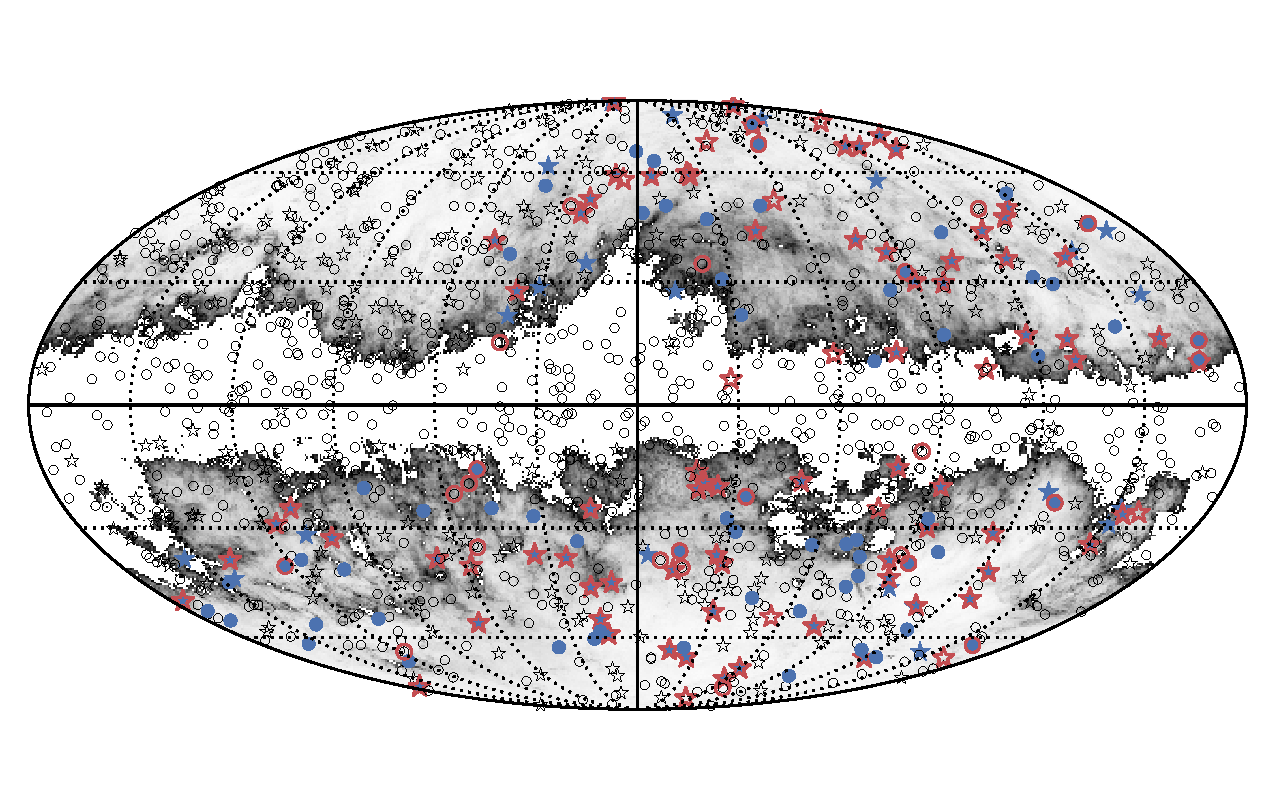
\includegraphics{figures/skymap.pdf}}
	\caption{Mollweide projection in galactic coordinates of the full sky showing
		the positions on the sky of the bursts presented in this work. The empty
		circles are the positions of all the \textit{Swift} bursts detected until the
		end of 2016. In blue is shown the position of the bursts fulfilling the sample
		criteria specified in Sect. \ref{samplecrit}. The red circles are added around
		GRBs which have been followed up by X-shooter since the commissioning of the
		instrument. Blue points with red circles represent GRBs that enter our sample
		and have X-shooter spectroscopy. The different samples are compared in Sect.
		\ref{results}. The background shows the dust maps presented in
		\citet{Schlegel1998} where the sample criteria cut with $A_V \lesssim 0.5$ mag
		is removed.}
	\label{fig:skymap}
\end{figure*}



Observations in this sample has been carried out using the cross-dispersed
echelle spectrograph, X-shooter \citep{Vernet2011}, mounted on two of the four
Unit Telescopes at ESO/VLT, UT2 (Kueyen) and UT3 (Melipal) during the duration
of this follow-up campaign, which covers the entire lifetime of X-shooter.
Observations have been carried out from the ESO period P84 through P98 under the
following programme IDs: 098.A-0055, 097.A-0036, 096.A-0079, 095.A-0045,
094.A-0134, 093.A-0069, 092.A-0124, 0091.C-0934, 090.A-0088, 089.A-0067,
088.A-0051, 087.A-0055, 086.A-0073, 085.A-0009 and 084.A-0260. A few additional
bursts, not a part of the \textit{statistical sample}, have been included from
092.D-0056(A) (PI: Rau), 092.D-0633(E) (PI: Greiner), and Levan under
095.B-0811(B) (PI: Levan). This sample represents \textit{all} GRBs that have
ever been followed up by X-shooter.

The first GRB followed up is GRB090313, observed 15th of March 2009, which was
while X-shooter was mounted on UT3 during the commissioning of the instrument.
The bursts observed during the commissioning period is not a part of our
statistical sample, but are nonetheless published as part of the bursts observed
by the X-shooter GRB team. The first burst observed after science verification
was completed when X-shooter was moved to UT2 is GRB091018 which thereby
constitute the first burst entering our statistical sample. For all bursts that
fulfill our sample selection criteria, described in Sect. \ref{samplecrit},
spectroscopic follow-up has been attempted with X-shooter. Various conditions
can affect our ability to follow up a given burst, and a discussion of this
effect is included in Sect. \ref{badbursts}.

X-shooter can cover the spectral wavelength region from 3000 \AA~to 24800 \AA~in
a single exposure, by splitting the light in three separate spectroscopic arms
using dichroics. This way each arm work as a separate instrument, each
functioning as its own echelle spectrograph. The ultraviolet blue(UVB) arm
covering 3000 - 5500 \AA, the visual(VIS) arm covering 5500 - 10200 \AA, and the
near-infrared()NIR) arm covering 10200 - 24800 \AA~ with the possibility of
applying a k-band blocking filter cutting the coverage of the NIR arm at 10200 -
21000 \AA. For all observations, a nod-and-shuffle observing scheme has been
employed, with a nodding throw of 5 \arcsec. The individual observations has
been carried out in a standard ABBA pattern, which allows flexibility in the sky
subtraction method for the different arms.

For the large majority of the bursts we have observed with a slit width of
1\farc0, 0\farc9, and 0\farc9 for the UVB, VIS, and NIR-arm respectively, which
puts a lower limit on the delivered resolution of the spectra based on the
tabulated values of the delivered resolutions, which is 4350, 7450, and 5300 for
the UVB, VIS and NIR-arm respectively\footnote{\url{https://www.eso.org/sci/facilities/paranal/instruments/xshooter/inst.html}}.
The slit width also sets the width of the atmospheric sky lines and determines
the amount of light lost due to the wavelength-dependent seeing PSF extending
outside the coverage of the slit, where the width of sky-lines is always set by
the slit width whereas both the delivered resolution and the slitloss changes
for the better as the seeing PSF drops below the slit width.
For atmospheric conditions delivering a seeing PSF with a FWHM of 0\farc9
observed with a 0\farc9 slit only 76.1 percent of the light will enter the slit,
meaning that for almost all observations a slitloss correction is required. We
describe how slitlosses were corrected for in Sect. \ref{postproc}.
For accurate measurements of velocity widths, a precise instrumental resolution
is required and this becomes better when the delivered seeing is better than the
slit width. We discuss this in Sect. \ref{resolution}.

Due to mechanical issues, the atmospheric dispersion corrector (ADC) were
disabled from 1st of August 2012. No bursts were affected by the failing ADC
prior to disablement. To avoid chromatic slit losses due to atmospheric
dispersion, all subsequent observations have been carried out at parallactic
angle. A consequence of this is that for all observations following 1st of
August 2012, the source moves across the spatial direction of the slit as a
function of wavelength. This effect has been modeled in the extraction
procedure, as described in \ref{extract}.

We list the overview of all the observations in Tab. \ref{tab:sample_overview}.
\LongTables
	
	\begin{deluxetable*}{@{\extracolsep{\fill}}lcccccclc@{}}
		%\tabletypesize{\scriptsize}
		%\rotate
		\tablecaption{The full sample of afterglows or hosts observed in the program.
			We here list the burst names and details of the spectroscopic observations. The
			exposure times and slit widths are given in the order UVB/VIS/NIR. The column
			$\Delta t$ shows the time after trigger when the spectroscopic observation was
			started. Mag$_\mathrm{acq}$ gives the approximate magnitude (typically in the
			$R$-band) of the afterglow in the acquisition image.
			\label{sample}}
		\tablewidth{0pt}
		\tablehead{
			\colhead{GRB} &  \colhead{Exptime} & \colhead{Slit width} & \colhead{Airmass} & \colhead{Seeing} & \colhead{$\Delta t$} & \colhead{Mag$_\mathrm{acq}$} & \colhead{Redshift} & \colhead{Ref}\\
			&  \colhead{(ks)}   & \colhead{(arcsec)} &   & \colhead{(arcsec)} & \colhead{(hr)}       &  & &  \\
		}
		\startdata
		GRB090313$^1$ 		& 6.9/6.9/6.9     	& 1.0/0.9/0.9 		& 1.2--1.4  	& 1.0  	&    45  	&  21.6  	& 3.3736 		& (1) \\
		GRB090530$^1$ 		& 4.8/4.8/4.8     	& 1.0/1.2/1.2 		& 1.6--2.2  	& 1.5  	&    20  	&  22    	& 1.266 		& (2) \\
		GRB090809$^1$ 		& 7.2/7.2/7.2     	& 1.0/0.9/0.9 		& 1.2--1.1  	& 0.9  	&  10.2  	&  21    	& 2.737  		& (2,3) \\
		GRB090926$^1$ 		& 7.2/7.2/7.2     	& 1.0/0.9/0.9 		& 1.4--1.5  	& 0.9  	&    22  	&  17.9  	& 2.1062 		& (4) \\
		GRB091018     		& 2.4/2.4/2.4     	& 1.0/0.9/0.9 		& 2.1--1.8  	& 0.8  	&   3.5  	&  19.1  	& 0.9710 		& (5) \\  
		GRB091127     		& 6.0/6.0/6.0     	& 1.0/0.9/0.9 		& 1.1--1.2  	& 1.0  	&   101  	&  21.2  	& 0.490  		& (6) \\
		GRB100205A     		& 10.8/10.8/10.8 	& 1.0/0.9/0.9 		& 1.9--1.8  	& 1.0  	&    71  	&   --   	&  --    		& (2) \\
		GRB100219A     		&  4.8/4.8/4.8   	& 1.0/0.9/0.9 		& 1.3--1.1  	& 0.7  	&  12.5  	&   23   	& 4.667  		& (7) \\
		GRB100316B     		&  2.4/2.4/2.4   	& 1.0/0.9/0.9 		& 2.0--2.4  	& 0.7  	&   0.7  	&  18.2  	& 1.18   		& (2) \\
		GRB100316D-1$^2$ 	&  7.2/7.2/7.2   	& 1.0/0.9/0.9 		& 1.2--1.5  	& 1.0  	&  12  		&   --   	& 0.059  		& (8) \\
		GRB100316D-2   		&  2.4/2.4/2.4   	& 1.0/0.9/0.9 		& 1.2--1.2  	& 1.0  	&    58  	&   --   	& 0.059  		& (8) \\
		GRB100316D-3   		&  2.4/2.4/2.4   	& 1.0/0.9/0.9 		& 1.2--1.2  	& 0.8  	&   192  	&   --   	& 0.059  		& (8) \\
		GRB100418A-1   		&  4.8/4.8/4.8   	& 1.0/0.9/0.9 		& 1.6--1.3  	& 0.7  	&   8.4  	&  18.1  	& 0.6235 		& (9) \\
		GRB100418A-2   		&  4.8/4.8/4.8   	& 1.0/0.9/0.9 		& 1.2--1.3  	& 0.6  	&    34  	&  19.2   	& 0.6235 		& (9) \\
		GRB100418A-3   		&  4.8/4.8/4.8   	& 1.0/0.9/0.9 		& 1.2--1.4  	& 0.7  	&    58  	&   --   	& 0.6235 		& (9) \\
		GRB100424A$^3$ 		&  4.8/4.8/4.8   	& 1.0/0.9/0.9 		& 1.1--1.2  	& 0.8  	&   --   	&   --   	& 2.465  		& (2) \\
		GRB100425A     		&  2.4/2.4/2.4   	& 1.0/0.9/0.9 		& 1.5--1.3  	& 0.7  	&   4.0  	&  20.6  	& 1.755  		& (2,3) \\
		GRB100621A     		&  2.4/2.4/2.4   	& 1.0/0.9/0.9 		& 1.3--1.4  	& 1.0  	&   7.1  	&   --   	& 0.542  		& (2) \\
		GRB100625A$^3$ 		&  4.8/4.8/4.8   	& 1.0/0.9/0.9 		& 1.1--1.0  	& 0.8  	&    13  	&   --   	& 0.452  		& (2) \\
		GRB100724A$^4$ 		&  4.2/4.2/4.2   	& 1.0/0.9/0.9 		& 1.5--2.3  	& 0.7  	&   0.2  	&   --   	& 1.288  		& (2) \\
		GRB100728B$^5$ 		&  7.2/7.2/7.2   	& 1.0/0.9/0.9 		& 1.5--1.1  	& 0.5  	&    22  	&   23   	& 2.106  		& (2) \\
		GRB100814A-1$^4$ 	& 0.9/0.9/0.9  		& 1.0/0.9/0.9 		& 1.9--1.7  	& 0.5  	&   0.8  	&   19   	& 1.44   		& (2) \\
		GRB100814A-2   		&  4.8/4.8/4.8   	& 1.0/0.9/0.9 		& 1.5--1.2  	& 0.6  	&   1.4  	&   19   	& 1.44   		& (2) \\
		GRB100814A-3   		&  4.8/4.8/4.8   	& 1.0/0.9/0.9 		& 1.2--1.0  	& 0.6  	&   99   	&   20   	& 1.44   		& (2) \\
		GRB100816A$^6$ 		&  4.8/4.8/4.8   	& 1.0/0.9/0.9 		& 1.8--1.6  	& 0.8  	&   3.7  	&   --   	& 0.806  		& (2) \\
		GRB100901A     		&  2.4/2.4/2.4   	& 1.0/0.9/0.9 		& 1.5--1.5  	& 1.8  	&   66   	&   --   	& 1.408  		& (10) \\
		GRB101219A     		&  7.2/7.2/7.2   	& 1.0/0.9/0.9 		& 1.1--1.7  	& 2.0  	&   3.7  	&   --   	& 0.718  		& (2) \\
		GRB101219B-1   		&  4.8/4.8/4.8   	& 1.0/0.9/0.9 		& 1.6--2.6  	& 1.3  	&  11.6  	&   20   	& 0.5519 		& (11) \\
		GRB101219B-2   		&  7.2/7.2/7.2   	& 1.0/0.9/0.9 		& 1.2--2.0  	& 0.8  	&   394  	&  22.7  	& 0.5519 		& (11) \\
		GRB101219B-3   		&  7.2/7.2/7.2   	& 1.0/0.9/0.9 		& 1.4--2.1  	& 0.9  	&   886  	&   --   	& 0.5519 		& (11) \\
		GRB110128A     		&  7.2/7.2/7.2   	& 1.0/0.9/0.9 		& 2.0--1.6  	& 0.9  	&   5.5  	&  22.5  	& 2.339  		& (2) \\
		GRB110407A     		&  9.6/9.6/9.6   	& 1.0/0.9/0.9 		& 1.4--1.3  	& 2.0  	&  12.4  	&   23   	&  --    		& (2) \\
		GRB110709B$^1,3$ 	&  7.2/7.2/7.2 		& 1.0/0.9/0.9 		& 1.6--1.1  	& 1.0  	&   --   	&   --   	&  --    		& (2) \\
		GRB110715A     		&  0.6/0.6/0.6   	& 1.0/0.9/0.9 		& 1.1--1.1  	& 1.7  	&  12.3  	&  18.5  	& 0.82  		& (2) \\
		GRB%110721A     	&  2.4/2.4/2.4   	& 1.0/0.9/0.9 		& 1.2--1.4  	& 2.4  	&        	&        	& 0.382  		& (2) \\
		GRB110808A     		& 2.4/2.4/2.4    	& 1.0/0.9/0.9 		& 1.2--1.1  	& 1.1  	&   3.0  	&  21.2  	& 1.3488 		& (2) \\
		GRB110818A     		& 4.8/4.8/4.8    	& 1.0/0.9/0.9 		& 1.3--1.3  	& 1.0  	&   6.2  	&  22.3  	& 3.36   		& (2) \\
		GRB111005A$^3$ 		& 1.2/1.2/1.2    	& 1.0/0.9/0.9 		& 1.3--1.3  	& 0.7  	&   --   	&  --    	& 0.013? 		& (2) \\
		GRB111008A-1   		& 8.8/8.8/8.4    	& 1.0/0.9/0.9 		& 1.1--1.0  	& 1.2  	&   8.5  	&  21?   	& 4.9898 		& (12) \\
		GRB111008A-2   		& 8.0/8.0/7.2    	& 1.0/0.9/0.9 		& 1.3--1.0  	& 1.0  	&  20.1  	&  22?   	& 4.9898 		& (12) \\
		GRB111107A     		& 4.8/4.8/4.8    	& 1.0/0.9/0.9 		& 1.8--1.5  	& 0.7  	&   5.3  	&  21.5  	& 2.893  		& (2) \\
		GRB111117A$^6$ 		& 4.8/4.8/4.8    	& 1.0/0.9/0.9 		& 1.5--1.4  	& 0.6  	&    38  	&  --    	& 1.3?   		& (2) \\
		GRB111123A-1   		& 6.2/6.6/6.6    	& 1.0/0.9/0.9 		& 1.6--1.1  	& 1.0  	&  12.2  	&  $>$24 	& 3.1516 		& (2) \\
		GRB111123A-2$^3$ 	& 2.4/2.4/2.4  		& 1.0/0.9/0.9 		& 1.0--1.0  	& 0.5  	&   --   	&  --    	& 3.1516 		& (2) \\
		GRB111129A     		& 3.6/3.6/3.6    	& 1.0/0.9/0.9 		& 1.6--2.1  	& 1.7  	&        	&        	&  --    		& (2) \\
		GRB111209A-1   		& 4.8/4.8/4.8    	& 1.0/0.9/0.9 		& 1.1--1.2  	& 0.8  	&  17.7  	&  20.1  	& 0.677  		& (13) \\
		GRB111209A-2   		& 9.6/9.6/9.6    	& 1.0/0.9/0.9 		& 1.2--2.0  	& 0.8  	&  497   	&  23    	& 0.677  		& (13) \\
		GRB111211A$^1$ 		& 2.4/2.4/2.4    	& 1.0/0.9/0.9 		& 1.4--1.6  	& 0.6  	&   31   	&  19.5  	& 0.478  		& (2) \\
		GRB111228A     		& 2.4/2.4/2.4    	& 1.0/0.9/0.9 		& 1.4--1.4  	& 0.9  	&  15.9  	&  20.1  	& 0.716  		& (2) \\
		GRB120118B$^3$ 		& 3.6/3.6/3.6    	& 1.0/0.9/0.9 		& 1.1--1.0  	& 1.0  	&   --   	&  --    	& 2.943  		& (2) \\
		GRB120119A-1   		& 2.4/2.4/2.4    	& 1.0/0.9/0.9 		& 1.1--1.1  	& 0.6  	&   1.4  	&   17   	& 1.728  		& (2) \\
		GRB120119A-2   		& 1.2/1.2/1.2    	& 1.0/0.9/0.9 		& 1.8--1.9  	& 0.6  	&   4.5  	&   20   	& 1.728  		& (2) \\
		GRB120119A-3$^3$ 	& 4.8/4.8/4.8  		& 1.0/0.9/0.6JH 	& 1.0--1.1  	& 1.1 	&   --   	&   --   	& 1.728  		& (2) \\
		GRB120211      		&                	&             		&           	&      	&        	&         	& 2.346 		& (2) \\
		GRB120224A     		& 2.4/2.4/2.4    	& 1.0/0.9/0.9 		& 1.7--2.1  	& 1.4  	&  19.8  	&   22.3 	&  --    		& (2) \\
		GRB120311A     		& 2.4/2.4/2.4    	& 1.0/0.9/0.9 		& 1.6--1.4  	& 0.6  	&   3.7  	&   21.6 	&  --    		& (2) \\
		GRB120327A-1   		& 2.4/2.4/2.4    	& 1.0/0.9/0.9 		& 1.6--1.4  	& 0.5  	&   2.1  	&   18.8 	& 2.815  		& (14) \\
		GRB120327A-2   		& 4.2/4.2/4.2    	& 1.0/0.9/0.9 		& 1.0--1.1  	& 1.0  	&    29  	&   22.5 	& 2.815  		& (14) \\
		GRB120404A     		& 9.6/9.6/9.6    	& 1.0/0.9/0.9JH 	& 1.7--1.3 		& 1.3 	&  15.7  	&   21.3 	& 2.876  		& (2) \\
		GRB120422A-1   		& 4.8/4.8/4.8    	& 1.0/0.9/0.9 		& 1.3--1.3  	& 0.6  	&  17.2  	&   22.0 	& 0.283  		& (15) \\
		GRB120422A-2   		& 4.8/4.8/4.8    	& 1.0/0.9/0.9 		& 1.3--1.4  	& 0.9  	&  113   	&   --   	& 0.283  		& (15) \\
		GRB120422A-3   		& 4.8/4.8/4.8    	& 1.0/0.9/0.9 		& 1.4--1.7  	& 1.0  	&  210   	&   --   	& 0.283  		& (15) \\
		GRB120422A-4   		& 4.8/4.8/4.8    	& 1.0/0.9/0.9JH 	& 1.3--1.4 		& 0.6  	& 449   	&   --   	& 0.283  		& (15) \\
		GRB120422A-5   		& 4.8/4.8/4.8    	& 1.0/0.9/0.9JH 	& 1.3--1.6 		& 0.8  	& 593   	&   --   	& 0.283  		& (15) \\
		GRB120422A-6   		& 4.8/4.8/4.8    	& 1.0/0.9/0.9JH 	& 1.7--2.4 		& 2.5  	& 882   	&   --   	& 0.283  		& (15) \\
		GRB120422A-7   		& 4.8/4.8/4.8    	& 1.0/0.9/0.9JH 	& 1.5--1.9 		& 1.3  	& 906   	&   --   	& 0.283  		& (15) \\
		GRB120712A     		& 4.8/4.8/4.8    	& 1.0/0.9/0.9   	& 1.5--2.5 		& 1.3  	& 10.4  	&   21.5 	& 4.175  		& (2) \\
		GRB120714B     		& 4.8/4.8/4.8    	& 1.0/0.9/0.9JH 	& 1.5--1.2 		& 1.2  	&  7.8  	&   22.1 	& 0.398  		& (2)\\
		GRB120716A$^1$ 		& 3.6/3.6/3.6    	& 1.0/0.9/0.9JH 	& 1.8--2.6 		& 1.0  	&  62   	&   20.9 	& 2.486  		& (2) \\
		GRB120722A$^2$ 		& 4.8/4.8/4.8    	& 1.0/0.9/0.9   	& 1.3--1.3 		& 1.1  	& 10.3  	&   23.6 	& 0.959  		& (2) \\
		GRB120805A$^2$ 		& 3.6/3.6/3.6    	& 1.0/0.9/0.9JH 	& 1.3--1.7 		& 0.9  	& 218   	&   --   	& 2.8?   		& (2) \\
		GRB120815A     		& 2.4/2.4/2.4    	& 1.0/0.9/0.9   	& 1.3--1.4 		& 0.6  	&  1.7  	&   20   	& 2.358  		& (16) \\
		GRB120909A     		& 1.2/1.2/1.2    	& 1.0/0.9/0.9   	& 1.6--1.6 		& 1.4  	&  1.7  	&   21   	& 3.929  		& (2) \\
		GRB120923A     		& 9.6/9.6/9.6    	& 1.0/0.9/0.9JH 	& 1.2--1.4 		& 1.0  	& 18.5  	&   --   	& $\gtrsim8$ 	& (2) \\
		GRB121024A     		& 2.4/2.4/2.4    	& 1.0/0.9/0.9   	& 1.2--1.1 		& 0.6  	&  1.8  	&   20   	& 2.300  		& (17) \\
		GRB121027A     		& 8.4/8.4/8.4    	& 1.0/0.9/0.9   	& 1.3--1.3 		& 0.9  	&  69   	&  21.1  	& 1.773  		& (2) \\
		GRB121201A     		& 4.8/4.8/4.8    	& 1.0/0.9/0.9JH 	& 1.1--1.1 		& 0.9  	& 12.9  	&   23   	& 3.385  		& (2) \\
		GRB121229A     		& 4.8/4.8/4.8    	& 1.0/0.9/0.9JH 	& 1.4--1.2 		& 1.4  	&  2.0  	&  21.5  	& 2.707  		& (2) \\
		GRB130131B$^3$ 		& 7.2/7.2/7.2    	& 1.0/0.9/0.9JH 	& 1.3--1.6 		& 0.8  	&  --   	&   --   	& 2.539  		& (2) \\
		GRB130408A     		& 1.2/1.2/1.2    	& 1.0/0.9/0.9   	& 1.0--1.0 		& 1.0  	&  1.9  	&   20   	& 3.758  		& (2) \\
		GRB130418A     		& 1.2/1.2/1.2    	& 1.0/0.9/0.9   	& 1.4--1.3 		& 1.3  	&  4.6  	&   18.5 	& 1.218  		& (2) \\
		GRB130427A     		& 1.2/1.2/1.2    	& 1.0/0.9/0.9JH 	& 1.8--1.8 		& 0.8  	& 16.5  	&   19   	& 0.340  		& (18) \\
		GRB130427B     		& 1.2/1.2/1.2    	& 1.0/0.9/0.9JH 	& 1.2--1.0 		& 0.8  	& 20.3  	&   22.7 	& 2.78   		&  (2) \\
		GRB130603B$^6$ 		& 2.4/2.4/2.4    	& 1.0/0.9/0.9   	& 1.4--1.4 		& 1.1  	&  8.2  	&   21.5 	& 0.356  		& (19) \\
		GRB130606A     		& 4.2/4.2/4.2    	& 1.0/0.9/0.9JH 	& 1.7--1.9 		& 1.1  	&  7.1  	&   19   	& 5.91   		& (20) \\
		GRB130612A     		& 1.2/1.2/1.2    	& 1.0/0.9/0.9   	& 1.3--1.3 		& 1.4  	&  1.1  	&   21.5 	& 2.006  		& (2) \\
		GRB130615A     		& 1.2/1.2/1.2    	& 1.0/0.9/0.9   	& 2.1--2.2 		& 1.0  	&  0.8  	&   21   	& $~3$?  		& (2) \\
		GRB130701A     		& 1.2/1.2/1.2    	& 1.0/0.9/0.9JH 	& 2.0--2.0 		& 1.6  	&  5.5  	&   19.9 	& 1.155  		& (2) \\
		\enddata
		\tablenotetext{1}{Not part of the statistical sample}
		\tablenotetext{2}{Spectrum dominated by light from the host galaxy}
		\tablenotetext{3}{Spectrum of the host galaxy taken long after the burst}
		\tablenotetext{4}{RRM observation}
		\tablenotetext{5}{ADC malfunction during observation}
		\tablenotetext{6}{Short burst}
		\tablerefs{
			(1) \citet{DeUgartePostigo2010}; (2) This work ; (3) Skuladottir (2010);
			(4) \citet{DElia2010}; (5) \citet{Wiersema2012}; (6) \citet{Vergani2011, Cobb2010}; 
			(7) \citet{Thone2013}; (8) \citet{Bufano2012} ; (9) \citet{DeUgartePostigo2011} ;
			(10) \citet{Hartoog2013}; (11) \citet{Sparre2011}; (12) \citet{Sparre2014};
			(13) \citet{Levan2014}; (14) \citet{DElia2014}; (15) \citet{Schulze2014};
			(16) \citet{Kruhler2013}; (17} \citet{Friis2015}
	\end{deluxetable*}
	%-------------------------END TABLE---------------------------------------
	 and plot the positions off all the bursts on
the night sky in Fig. \ref{fig:skymap}. The central zone of avoidance due to
high galactic extinction cutoff is visible with an apparent isotropic
distribution of the bursts away from the galactic center except in the upper
right corner, where Earth casts a shadow on the sky as seen from the telescope.

A subset of the bursts presented here  have already had their hosts investigated
in \citet{Kruhler2015}, for which extractions of the hosts exist. The focus of
the data presented here are on the afterglows themselves and in the absence of a
clear afterglow, the host. We will not, however, investigate the hosts.

%%%%%%%%%%%%%%%%%%%%%%%%%%%%%%%%%%%%%%%%%%%%%%%%%%%%%%%%%%%%%%%%%%%%%%%%%%%%
\section{Data processing}
%%%%%%%%%%%%%%%%%%%%%%%%%%%%%%%%%%%%%%%%%%%%%%%%%%%%%%%%%%%%%%%%%%%%%%%%%%%%

In this section we describe how the final data products are produced and
subsequently post-processed. $\sim$ 30 percent of the data released here have
been reduced in a manner similar to what is described in \citet{Kruhler2015}.
The two reduction schemes have been tested and are in good agreement. All
post-processing scripts developed for this dataset are made publicly available
at \url{https://github.com/jselsing/XSGRB_reduction_scripts}, along with
instructions of use.

Before any reductions are done, the raw object images are run through the
cosmic-ray removal algorithm \citep{VanDokkum2001} implementation,
\textit{Astro-SCRAPPY} \footnote{\url{https://github.com/astropy/astroscrappy}},
where a wide clipping radius have been used around detected cosmics to ensure that edge residuals are
robustly rejected. 

The basis for the reductions is the VLT/X-shooter pipeline, version
\texttt{2.7.1} or newer \citep{Goldoni2006, Modigliani2010}. The pipeline is
managed with the Reflex interface \citep{Freudling2013} and is used for
subtraction of bias level, flat-fielding, tracing of the echelle orders,
wavelength calibrations with the use of arc-line lamps, flux calibration using
spectrophotometric standards \citep{Vernet2010, Hamuy1994}, mirror flexure
compensation, initial sky-subtraction and lastly the rectification and merging
of the orders. For the initial sky-subtraction, the background has been
estimated in regions adjacent to the object trace clear of contaminating
sources. Because of the broken ADC, for some objects there is a lot of curvature
in the object trace. This means that for some bursts, the initial sky-estimate
has been made from a limited number of pixels in the spatial direction. By doing
an initial subtracting the sky on the un-rectified image we ensure that bulk of
the sky background is not redistributed by the rectification process.

The image is rectified onto an equidistant grid with a dispersion sampling of
0.2 \AA/pixel and a 0.16 "/pixel spatial sampling for the UVB and VIS arm and
0.6 \AA/pixel with a 0.21 "/pixel in the NIR arm.  Because the tabulated
resolution is a lower limit, by choosing a sampling of 0.2 \AA/pixel, we ensure
that the bluest part of neither of the arms have a sampling lower than the
Nyquist sampling rate of 2 pixels per resolution FWHM.

%%%%%%%%%%%%%%%%%%%%%%%%%%%%%%%%%%%%%%%%%%%%%%%%%%%%%%%%%%%%%%%%%%%%%%%%%%%%
\subsection{Post-processing} \label{postproc}
%%%%%%%%%%%%%%%%%%%%%%%%%%%%%%%%%%%%%%%%%%%%%%%%%%%%%%%%%%%%%%%%%%%%%%%%%%%%

For a typical observation, each of the exposures in the nodding sequence has
been reduced as single observation and then subsequently combined to form a
single image. Because this strategy is employed, we can reject outliers in the
stack and weight by the average inverse variance of the background. When
weighting images where the noise in each pixel is dominated by Poisson noise it
important to estimate the background variance in a large enough region, so that
to remove the correlation between the signal and the weights. To this end, the
weight map is generated by a running median window over the variance map, where
the trace as been masked and width of the window is chosen to be wide enough for
median variance to be generated on the basis of several hundred pixels. This
weighting scheme automatically also optimally combines images of different
exposure times or images where the background is varying, which is often the
case when a burst has been observed close to twilight

Because the background is very bright and there is a high abundance of broad
sky-lines in the NIR arm, when there are no contaminating sources in the slit,
the sky has been put back on the images and they have been reduced in pairs of
two, subtracting the two from each other, keeping the WCS static. This amounts
to the regular nodding reduction, only we can reject outliers and weight by the
averaged inverse variance map.

By STARE reducing all observations we additionally get a spectrum of the sky,
which we can use to calibrate the wavelength solution in Sect. \ref{wavecal}.


%%%%%%%%%%%%%%%%%%%%%%%%%%%%%%%%%%%%%%%%%%%%%%%%%%%%%%%%%%%%%%%%%%%%%%%%%%%%
\subsection{Correction for offsets in the wavelength calibration}    \label{wavecal}
%%%%%%%%%%%%%%%%%%%%%%%%%%%%%%%%%%%%%%%%%%%%%%%%%%%%%%%%%%%%%%%%%%%%%%%%%%%%

X-shooter, being installed at the VLT Cassegrain focus is  prone to flexures
during operations. The flexures modify the projection of the slit on the
detector with respect to the one obtained in daytime calibration. This requires a
modification of the wavelength solution in order to process correctly the
night-time data. Part of this correction is performed by the pipeline using the
frames taken during X-shooter Active Flexure Compensation procedure
\footnote{X-shooter User Manual available at
	https://www.eso.org/sci/facilities/paranal/instruments/xshooter/doc.html}.

The remaining offset is corrected by cross-correlation with a synthetic sky
spectrum \citep{Noll2012, Jones2013} after the continuum, estimated as the mode
of all flux values, has been subtrated. To get the correct seeing PSF with which
to convolve the synthetic sky an initial refinement of the wavelength solution
have been obtained by cross-correlating the observed sky with an unconvolved
synthetic sky. This preliminary wavelength calibration is applied to the
observed sky. The synthetic spectrum is then convolved with an increasing seeing
PSF and the width that minimizes $\chi^2$ with the updated observed sky is
chosen to be the effective sky-PSF. Using the synthetic sky with the matched
resolution, a final wavelength calibration can then be calculated by
cross-correlating the observed sky with the correctly broadened sky spectrum, as
a function of a velocity offset. Both a multiplicative and an additive offset to
the wavelength calibration has been tested, but in terms of $\chi^2$, the model
with only a multiplicative offset is preferred.

The resulting offsets, which were smaller than 0.1 \AA~in the UVB and VIS data
and smaller than 0.5 \AA~in the NIR spectra, but changing over short period of
time were applied to the corresponding spectra.

Using the convolved synthetic sky, the $\gtrsim 3 \sigma$ sky brightness pixels
have been added to the bad pixel map to avoid the cores of the brightest
sky-lines.

%%%%%%%%%%%%%%%%%%%%%%%%%%%%%%%%%%%%%%%%%%%%%%%%%%%%%%%%%%%%%%%%%%%%%%%%%%%%
\subsection{Spectral extraction}    \label{extract}
%%%%%%%%%%%%%%%%%%%%%%%%%%%%%%%%%%%%%%%%%%%%%%%%%%%%%%%%%%%%%%%%%%%%%%%%%%%%

To extract the afterglow spectrum from the rectified 2D-image, several
techniques have been employed based on the brightness of the afterglow and the
complexity of the objects entering the slit. Due to the malfunctioning ADC, see
Sect. \ref{obs}, the spectral trace moves across the slit as a function of
wavelength for a large fraction of the bursts observed meaning that using a
single aperture for the spectral extraction is inadequate due to the large
amount of background that would then enter the slit. To optimally select the
extraction regions we therefore need to model the trace position.

To get the shape and the position of the spectral PSF as a function of location
on the image, we need to chose a model which can represent how the light falls
on the slit. We know from \citet{Trujillo2001} that the Moffat function
\citep{Moffat1969} adequately describes an imaging PSF due to atmospheric
turbulence, but due to the aberrations in the dispersion elements and the
rectification process, the PSF we are trying to model different from this
profile. To allow for flexibility in the model, we have chosen the Voigt
function as a model for the spectral PSF and we describe how this is evaluated
in App. \ref{voigt}. Since additionally, the host galaxy could also have a
contribution the image profile, this choice allows for the required freedom if
additional flux is in the wings of the profile.

To guide the guess position of the trace on the slit as a function of
wavelength, we have used the analytic prescription for the trace position
described in \citet{Filippenko1982}, where the header keywords of the
observations have been queried for the ambient conditions which controls the
degree to which the trace moves.

Based on the signal-to-noise of the afterglow continuum, the 2D-image has been
binned down in the spectral direction to a number of elements that allows for an
accurate tracing of the PSF, typically 200 bins for moderate signal-to-noise.
For each of the bins and using the guess position, the spectral PSF has been fit
using the unweighted chi-squared minimization algorithm implemented in
\texttt{scipy.optimize.curve\_fit} \citep{scipy}. Since we know that the trace
varies slowly as a function of wavelength, we have then fitted a low-order
polynomial to the fit parameters as a function of wavelength, which allows us to
evaluate the spectral PSF at all wavelengths and this way accurately model the
entire spectral PSF.

Equipped with a model for how the light falls on the entire image, we can then
employ the optimal extraction algorithm \cite{Horne1986}, which weights the
extraction aperture by the spectral profile, or alternatively sum all pixels
within 1 FWHM of the modeled profile. Where possible, we have used the optimal
extraction. In cases where the trace is very weak, even in the binned images, an
aperture has been selected manually which covers emission lines, if present, and
when nothing is immediately visible, the entire nodding window. The error- and
bad pixel maps are in all cases propagated throughout the extraction.

In cases where multiple traces are visible in the slit, additional components
for the profile are used in the optimal extraction. The additional components
do not share the PSF parameters and in cases where the additional component is an
extended object, the fits have been inspected to ensure that the additional
component does now skew the fit towards a different PSF. The additional
components are not used for the weights.

The spectra are corrected for galactic extinction using the E(B-V) value from
the dust maps of \citet{Schlegel1998} with the update in
\citet{Schlafly2011}\footnote{Queried from
	http://irsa.ipac.caltech.edu/applications/DUST/index.html using
	\citet{astroquery}}, and the extinction curve by \cite{Cardelli1989} with a
total to selective extinction $R_V = 3.1$. The wavelengths of the extracted
1D-spectra are moved to vacuum, moved to the barycentric frame, and the
wavelength recalibration described in Sect. \ref{wavecal} is applied. Pixels
with pixel-to-pixel variation large than $50 \sigma$ are added to the bad pixel
map.


%%%%%%%%%%%%%%%%%%%%%%%%%%%%%%%%%%%%%%%%%%%%%%%%%%%%%%%%%%%%%%%%%%%%%%%%%%%%
\subsection{Telluric correction} \label{tell_corr}
%%%%%%%%%%%%%%%%%%%%%%%%%%%%%%%%%%%%%%%%%%%%%%%%%%%%%%%%%%%%%%%%%%%%%%%%%%%%

For all earth-based telescopes, the light of interest has to pass through Earths
atmosphere, where the atmospheric content and conditions make an imprint on the
received spectrum. These telluric features can be corrected for in a multitude
of ways. We employ a prioritized list of methods here, depending on the
availability of the different method. Since the observation are often taken at
odd times under varying conditions, this prioritized list ensures that we are
always doing the optimal correction.

The highest priority method is using the GRB afterglow continuum itself, where
the atmospheric conditions have directly been imprinted on the spectrum. The
telluric features can directly be fit with an atmospheric model
\citep{Smette2015, Kausch2015}, which can then be used to correct for the
absorption. The accuracy of the correction depends on the S/N for the target
spectrum, where we have chosen the requirement that the afterglow continuum
spectrum has a median signal-to-noise higher than a value of 10.

If the afterglow is not sufficiently bright, telluric standard stars observed
close in the time to the GRB can be used as a proxy for the atmospheric
condition during the GRB observation. Here we employ the telluric correction
method that has been developed in \citet{Selsing2015}, where a library of
synthetic templates is fit to the observed telluric standard.

In the last case, where the object is neither bright enough, or there for some
reason have not been observed a telluric standard, we rely on the synthetic sky
model by \citep{Noll2012, Jones2013} for which we generate a synthetic
transmission spectrum, which we then use, where the ambient parameters for the
observations have been used.


\begin{figure*}
	\centerline{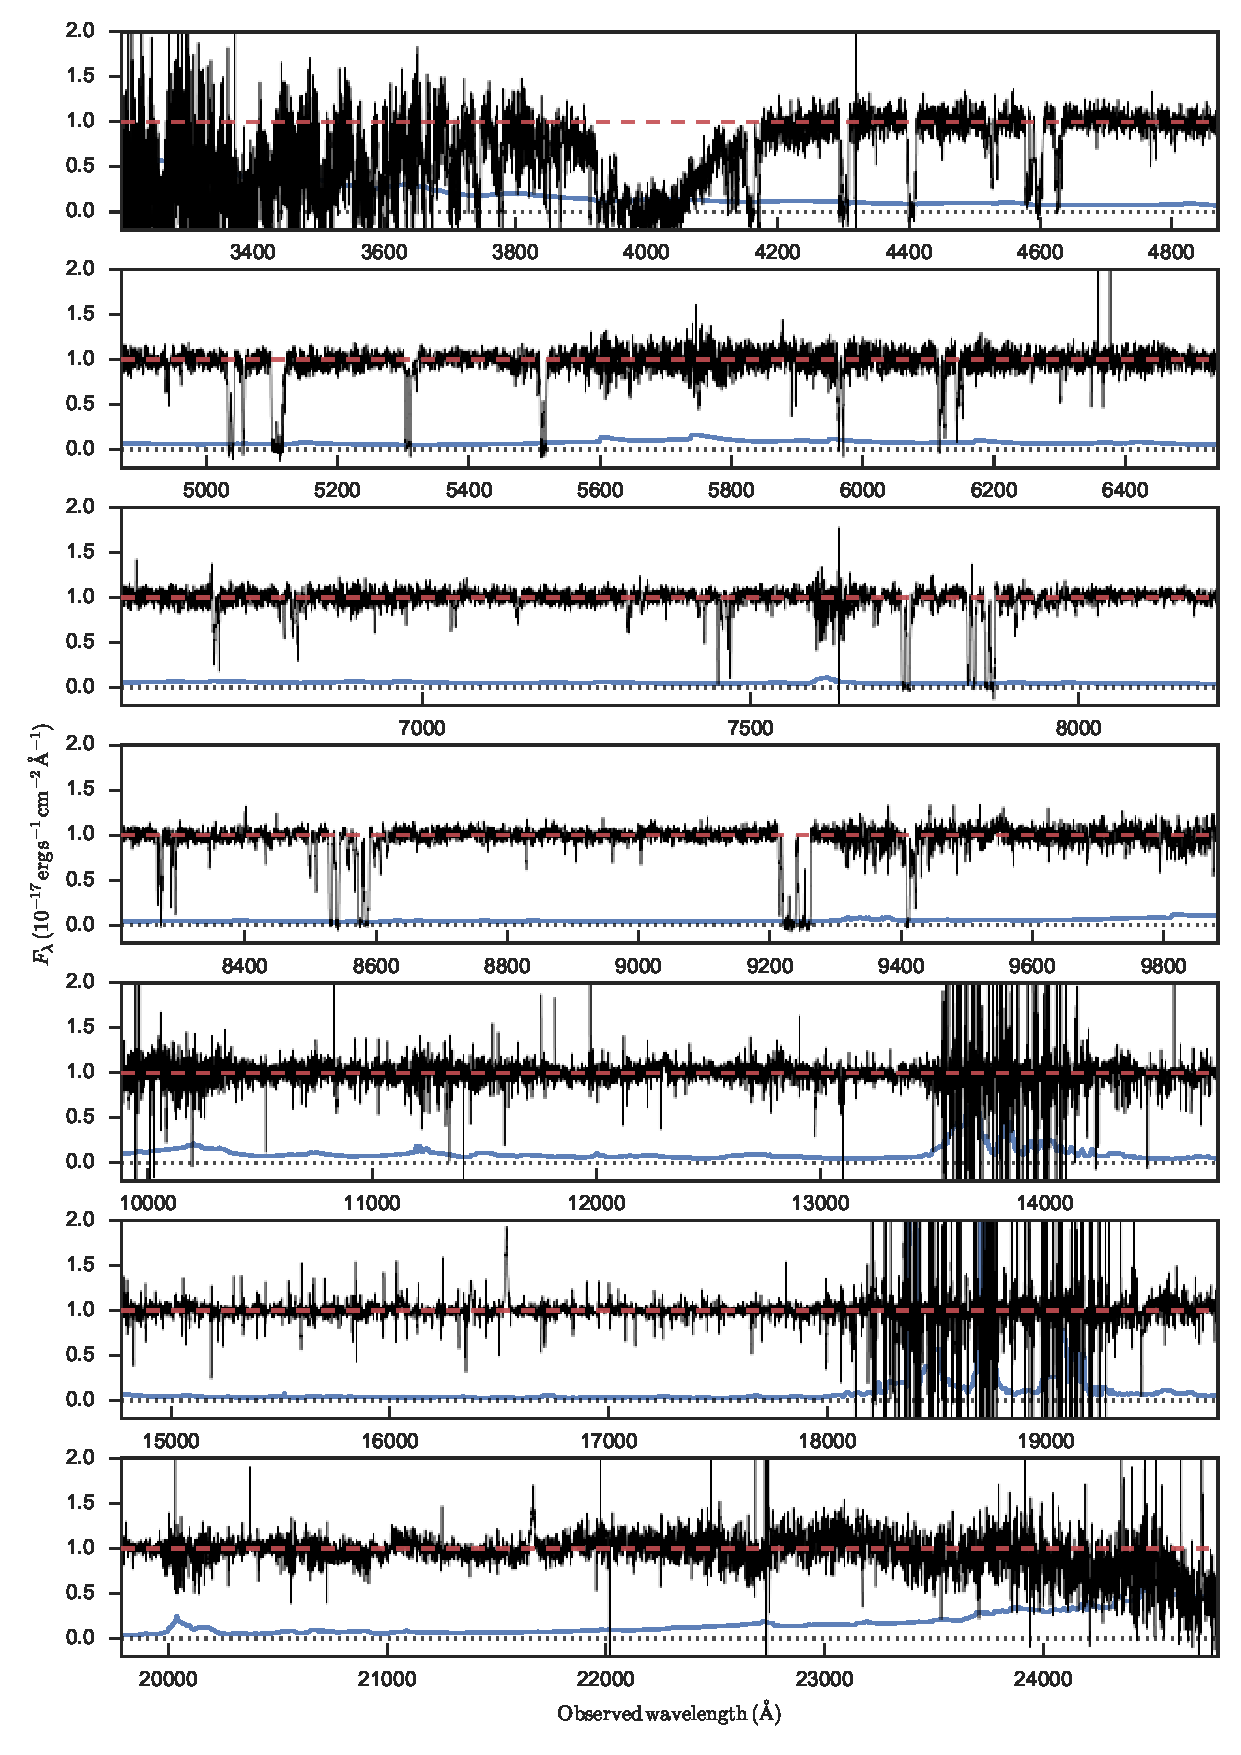
\includegraphics[width=0.85\linewidth]{figures/GRB121024A.pdf}}
	\caption{Telluric corrected, normalized spectrum of GRB121024A at $z = 2.300$,
	meant to illustrate the typical data quality. The acquisition magnitude is r =
	20, meaning it is in the brighter end of the sample presented here, but not the
	brightest. The spectrum is rich in absorption, including molecular absorption
	of $H_2$. The absorption trough visible at $\sim$ 4000 $\AA$ is due to \lya in
	the host. We have overplot the most prominent lines seen in GRB afterglows from
	\citet{Christensen2011a}. The continuum estimate is shown in dashed red.
	Additionally, three intervening systems are seen in this sightline  This
	spectrum has been analyzed in detail in \citet{Friis2015}.}
	\label{fig:spectrum}
\end{figure*}


%%%%%%%%%%%%%%%%%%%%%%%%%%%%%%%%%%%%%%%%%%%%%%%%%%%%%%%%%%%%%%%%%%%%%%%%%%%%
\subsection{Spectral resolution} \label{resolution}
%%%%%%%%%%%%%%%%%%%%%%%%%%%%%%%%%%%%%%%%%%%%%%%%%%%%%%%%%%%%%%%%%%%%%%%%%%%%


\begin{figure}[!ht]
	\centerline{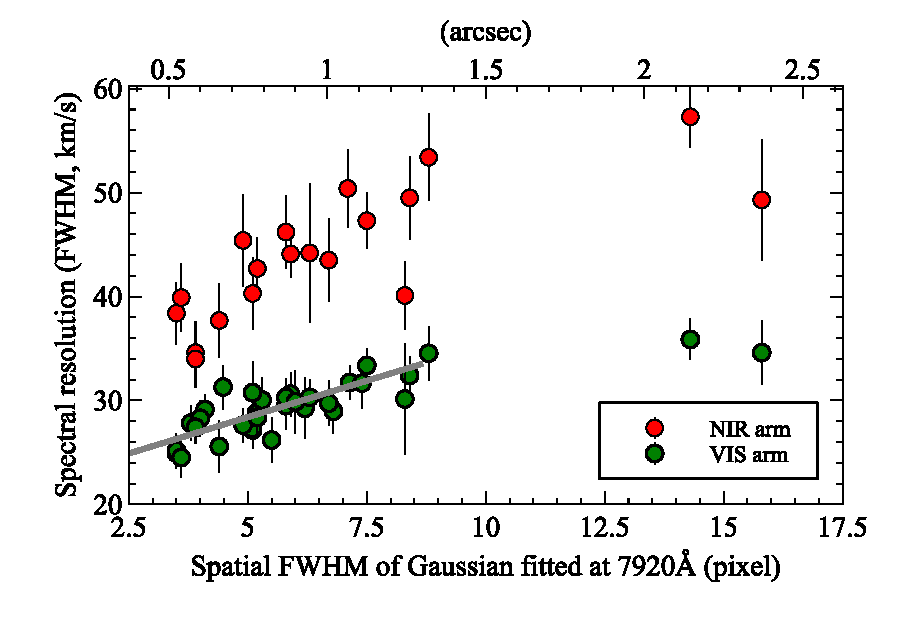
\includegraphics[width=8cm]{figures/resolution_paper.eps}}
	\caption{Green datapoints show the FWHM (km/s) of Gaussian fits to unresolved telluric absorption lines in the VIS spectra, as a function of the FWHM of a Gaussian fit onto the trace in spatial direction at  792 nm. The lower horizontal axis is in units pixels, the top axis in arc seconds. The red datapoints show a subsample of NIR spectra.
		The grey line shows a linear fit to the VIS datapoints. }
	\label{fig:res}
\end{figure}


The afterglow spectra described in this paper are obtained in
Target-of-Opportunity (override) mode.
In most cases there is therefore little possibility to tweak slit widths to the
seeing at the time of observations (i.e. to optimise spectral resolution and
signal to noise), and almost all our data is therefore taken with a fixed set
of slit widths and binning, described above.
In a fair number of cases, the seeing full width at half maximum (FWHM) is
considerably smaller than the silt width, and the delivered spectral resolution
will then be determined by the seeing rather than slit width, as afterglows are
point sources (this is evidently not the case for extended sources, e.g for
host galaxies).
The delivered resolution for slit width dominated spectra post-reduction and
extraction can easily be determined from the bright sky emission lines.
For afterglow spectra with very high signal to noise, the delivered spectral
resolution can at times be determined from the science data themselves.
However, in the presence of multiple velocity components in absorption, other
forms of line broadening, and a lack of lines at some redshifts, this is
difficult to do at poorer signal to noise ratios (the majority of spectra in
our sample).
A broad starting value for the expect resolution will help fitting of these
spectra, and can be important in upper limit determination, and for this reason
we construct a aim to construct a crude relation between the seeing and the
delivered resolution at our slit width, binning, and reduction pipeline
settings.
To this end we use observations of telluric standard stars that are taken with
identical instrument settings as our afterglow spectra, usually just after the
science data, as part of the ESO X-shooter calibration plan.
These spectra have been reduced together with the afterglow spectra, using
identical pipeline settings with the same version of the pipeline.
First we fit a Gaussian function in the spatial direction of the trace of the
standard star at 792 nm (i.e. in the VIS arm).
After this, we fit a series of  20 telluric absorption lines in the telluric
standard star spectra with Gaussians, taking care to select transitions that
are not almost-resolved multiples, should be intrinsically unresolved, and are
in areas with well defined continuum flux.
We pick 34 telluric standard stars spanning a range of DIMM seeing values, with
the majority between $0.5-1.5 arcsec$.
The resulting distribution of spectral FWHM (km/s) as a function of spatial
FWHM at 792 nm is fairly well described by a linear relation $a + b*x$, with
$x$ the spatial FWHM in pixels (with 0.15 arc sec per pixel),  $a= 21.4 \pm
1.3$ km/s, $b=1.4 \pm 0.2$.
We use this linear relation as a way to estimate the spectral resolution for
medium to poor signal to noise afterglow spectra in the VIS arm.
To extend this to the UVB and NIR arm, we measured a series of lines in NIR arm
spectra of a subset of 19 sources used for the VIS arm above, and find that the
resulting distribution is consistent with a simple scaling of the VIS arm
relation by the ratio of resolutions of the NIR and VIS arm for unresolved,
slit filling, sources as given on the ESO instrument website.
The UVB arm contains no suitable absorption lines to use, and we therefore use
a scaled value as in the NIR arm.
While this simple method is not terribly accurate (for one, the spatial profile
of the trace is not a perfect Gaussian), but it gives a sufficiently accurate
estimate for the analysis of these poor signal to noise science spectra.


%%%%%%%%%%%%%%%%%%%%%%%%%%%%%%%%%%%%%%%%%%%%%%%%%%%%%%%%%%%%%%%%%%%%%%%%%%%%
\subsection{Science data products} \label{products}
%%%%%%%%%%%%%%%%%%%%%%%%%%%%%%%%%%%%%%%%%%%%%%%%%%%%%%%%%%%%%%%%%%%%%%%%%%%%

In this section we describe the data format. Similar to what is done in \citet{Lopez2016}





%%%%%%%%%%%%%%%%%%%%%%%%%%%%%%%%%%%%%%%%%%%%%%%%%%%%%%%%%%%%%%%%%%%%%%%%%%%%
\section{Results} \label{results}
%%%%%%%%%%%%%%%%%%%%%%%%%%%%%%%%%%%%%%%%%%%%%%%%%%%%%%%%%%%%%%%%%%%%%%%%%%%%

In this section we describe the efficiency of the follow-up effort and the
characteristics of the observed bursts. We also assess the degree to which the
sample obtained is complete. An important note is that here we present
\textit{all} GRBs that have ever been observed with X-shooter, while only a
subset of these constitute our \textit{statistical} sample. The statistical
sample is based on the selection criteria described in Sect. \ref{samplecrit}
and should represent an unbiased sample of the underlying, parent GRB
population. Single bursts outside the sample criteria have been followed up on
the basis of the curiosity of their light curve or their brightness, but is not
discussed as part of the investigation of the GRB population. A prime example of
a burst outside the statistical sample is GRB161023A with it's rich
spectrum containing 11 intervening absorption systems and pending further analysis. 


%%%%%%%%%%%%%%%%%%%%%%%%%%%%%%%%%%%%%%%%%%%%%%%%%%%%%%%%%%%%%%%%%%%%%%%%%%%%
\subsection{Follow-up timing and afterglow brightness} \label{timing}
%%%%%%%%%%%%%%%%%%%%%%%%%%%%%%%%%%%%%%%%%%%%%%%%%%%%%%%%%%%%%%%%%%%%%%%%%%%%

Redshift determination of bursts where the host is too faint for a spectroscopic
redshift relies on the absorption spectrum imprinted on the GRB afterglow
continuum, which again depends on the afterglow brightness at time of follow-up.
Because the afterglow rapidly fades \citep{Nousek2006, Vecchio2016}\todo{Better references} a rapid
follow-up is essential for the accurate designation of the GRB host \todo{Get
reference}. In Fig. \ref{fig:timing} we plot the follow-up delay from the BAT
trigger to the start of the spectroscopic observation. Visible as the
shortest delays are the bursts observed in RRM-mode in which where the fastest follow-up
between BAT trigger and start of spectroscopic observations is for the short, $z = 1.717$, GRB160410A which was
followed up only 8.4 minutes after the BAT trigger.


\begin{figure}
	\centerline{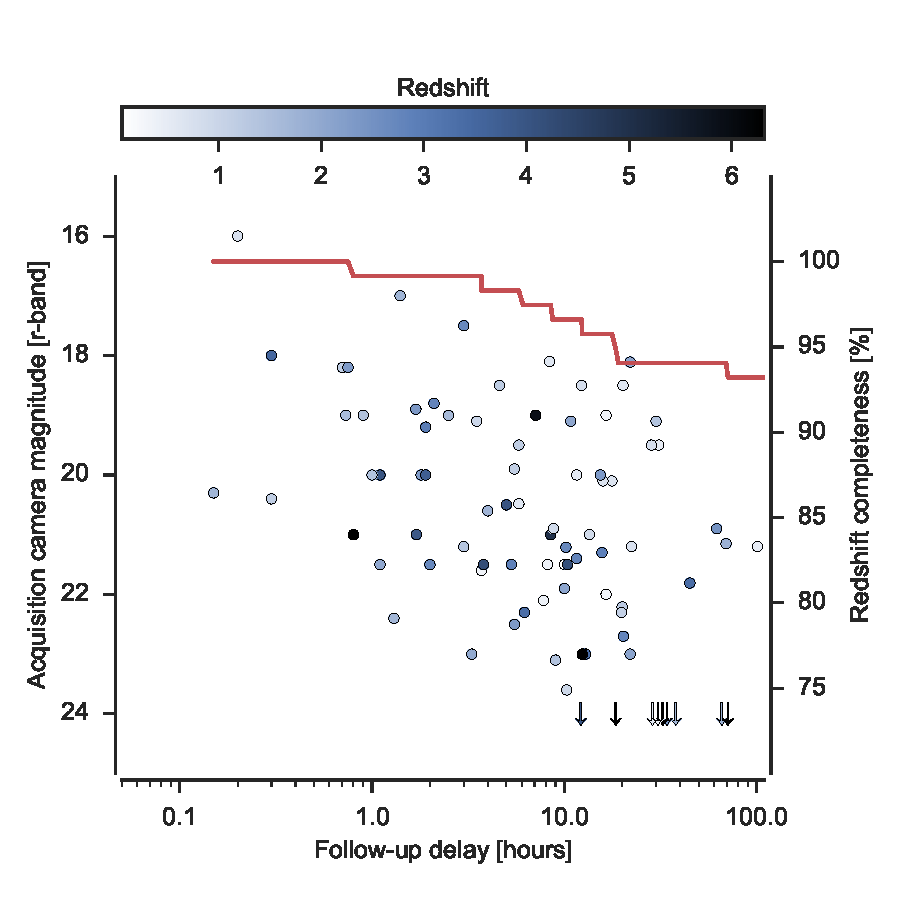
\includegraphics[width=8cm]{figures/timing.pdf}}
	\caption{Follow-up timing and afterglow magnitude at the start of observation.
	The points have been colored based on the redshift of the corresponding burst.
	Points with black faces does not have a redshift determination and downarrows
	indicate a non-detection in the acquisition image. In blue is shown the
	fractional redshift completess as a function of delay-time.}
	\label{fig:timing}
\end{figure}

To illustrate the effect of redshift completeness loss due to late follow-up, we
overplot the redshift completeness fraction over the delay time. Visible is the
increasing fraction of GRBs without a good redshift determination for increasing
delays. That the redshift completeness of the bursts we have followed up are $>$
90 percent \todo{Get number}, shows the ability of VLT/X-shooter to successfully
get redshifts. Not shown in the figure is an additional 12 \todo{Get number}
bursts that we have redshift determinations from late-time host observations
with delay-times longer than $\sim$10 days.


%%%%%%%%%%%%%%%%%%%%%%%%%%%%%%%%%%%%%%%%%%%%%%%%%%%%%%%%%%%%%%%%%%%%%%%%%%%%
\subsection{Sample completeness} \label{completeness}
%%%%%%%%%%%%%%%%%%%%%%%%%%%%%%%%%%%%%%%%%%%%%%%%%%%%%%%%%%%%%%%%%%%%%%%%%%%%

Based on the sample criteria specified in Sect. \ref{samplecrit}, a total of 158
\todo{Get number} bursts has been triggered by \textit{Swift} in the period
since the commissioning of VLT/X-shooter in November, 2009. This sample
constitutes the \textit{statistical sample} on which we will try to address the
GRB population properties. Of this sample, 86 \todo{Get number} have been
spectroscopically followed up with X-shooter. In order to assess whether our
sample criteria and the subset of bursts followed up represent the underlying
parent population of GRB, we compare some intrinsic GRB properties of our sample
to the full sample of GRBs followed up by \textit{Swift}. Under the assumption
that \textit{Swift} randomly samples the underlying GRB population, if the
sample statistics of our subsample are similar to the \textit{Swift}-sample, we
can assume that the population properties should be conserved. There is some
evidence that the burst duration does not scale with redshift as expected
through time-dilation\citep{Kocevski2013, Littlejohns2013a}, pointing towards
that we could be missing an increasing fraction of the bursts at higher
redshifts, but \citet{Lien2016} argues that we should only be missing the bright
"short" GRBs", but to the degree that \textit{Swift} is complete, we can test if
the sample presented here is complete. We show the comparison between the burst
properties in Fig. \ref{fig:swift_complete}.


\begin{figure*}
	\centerline{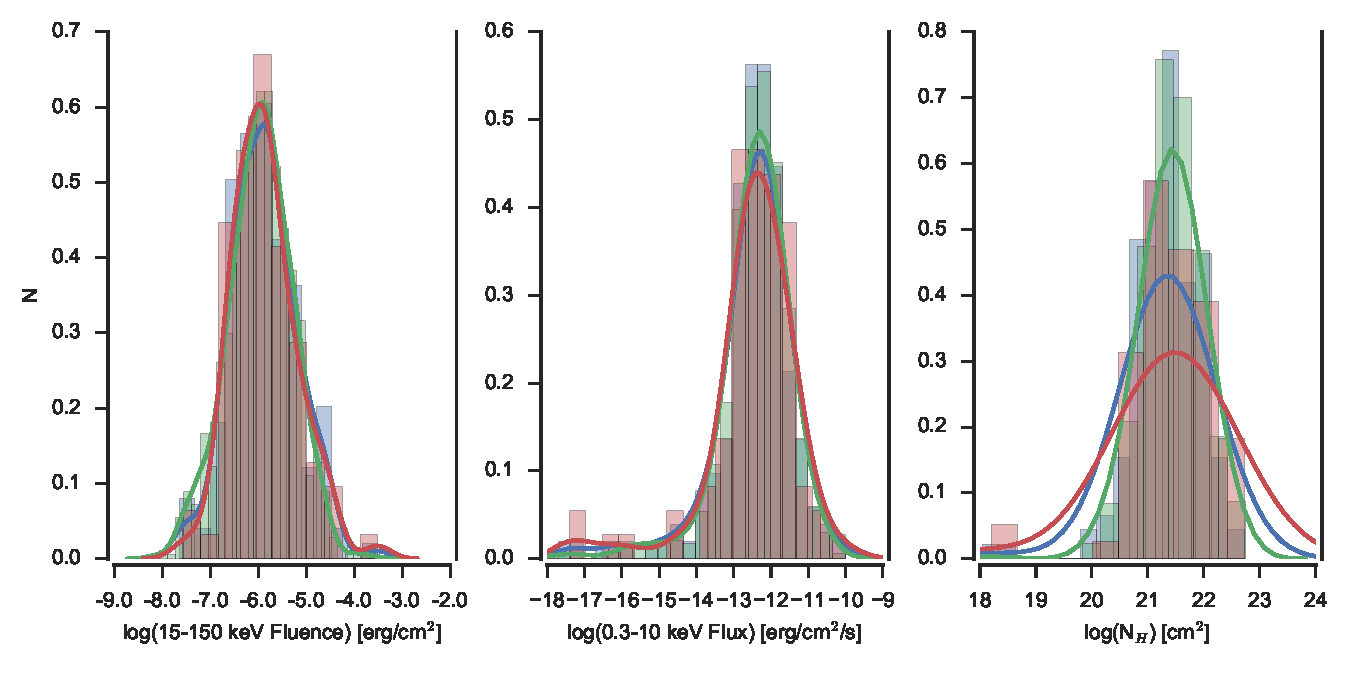
\includegraphics[width=18cm]{figures/completeness_BAT.pdf}}
	\caption{Comparison between bursts properties of all bursts observed with
	\textit{Swift}, the properties of the ones that fullfill the sample criteria
	specified in Sect. \ref{samplecrit}, and the subset that has been observed as
	part of the statistical sample. The left plot shows the fluence in 15-150 keV
	as observed by BAT. The middle panel shows the 0.3 - 10 keV flux, 11 hours
	after the bursts as measured by XRT. Based on the XRT spectrum,
	\citep{Evans2009}, a hydrogen column density has been inferred which we show in
	the right most panel.}
	\label{fig:swift_complete}
\end{figure*}

Using the observational characteristics of the 1244 \todo{Get number} bursts
observed by \textit{Swift} to date \cite{Gehrels2009}, and the X-ray derived
hydrogen column densities \citep{Evans2009}, we can quantify the degree to which
our sample is biased against the overall \textit{Swift} sample in terms of
intrinsic GRB properties. The values are queried from the online \textit{Swift}
database maintained\footnote{http://swift.gsfc.nasa.gov/archive/grb\_table/}.
Three main samples are of interest to compare to assess the completeness of the
follow-up campaign; the full \textit{Swift} sample consisting of all the bursts
observed by \textit{Swift}, excluding the bursts entering our sample (1), the
burst that fulfill the selection criteria imposed in Sect. \ref{samplecrit}, but
has not been followed up (2), and the bursts actually followed up with X-shooter
(3).

\begin{table*}[!ht]
	\centering
	\begin{tabular}{cccc}
		\hline
		\hline\noalign{\smallskip}
		{} & {Full \textit{Swift} sample} & {Statistical sample} &  {Followed up bursts} \\
		\hline\noalign{\smallskip}
		N$_{BAT}$ & 981 & 163 & 92\\
		$\log(15-150$keV fluence)  & $-5.9_{-0.6}^{+0.7}$ &  $-5.9_{-0.6}^{+0.7}$ &  $-5.9_{-0.7}^{+0.7}$   \\
		N$_{XRT}$ & 902 & 160 & 90\\
		$\log(0.3-10$keV flux) & $-12.3_{-0.8}^{+0.7}$ &  $-12.4_{-0.8}^{+0.7}$ &  $-12.4_{-0.7}^{+0.9}$  \\
		N$_{\mathrm{HI_x}}$ & 248 & 99 & 79\\
		$\log(\mathrm{N}_{\mathrm{HI_x}})$ & $21.7_{-0.9}^{+0.6}$ &  $21.5_{-3.4}^{+0.7}$ &  $21.6_{-4.5}^{+0.7}$  \\
		\hline\noalign{\smallskip}

\end{tabular} 

\caption{
	Population properties (median and 14th and 86th percentiles as the
	error intervals) for the \textit{Swift sample} and the subset of bursts
	fulfilling the sample criteria. The population characteristics of the three
	samples are very similar, which shows that our selection criteria effectively
	conserve the statistical properties of the underlying population, as least for
	these parameters.  Notice that not all bursts have measurements of the
	quantities we compare. \label{tab:sample_properties}
	}

\end{table*}

For each of the samples we calculate the median and 14th and 86th percentile
which can be used as point estimates for the population distribution. These are
shown in \ref{tab:sample_properties}. It can be seen from the values that the
three samples have very similar distributions in terms of the point estimates
chosen, suggesting that our selection criteria are unbiasing against the
\textit{Swift}-sample and that additionally, the follow-up effort is unbiasing
towards the intrinsic GRB properties. This is despite spectroscopic follow-up
only being carried out in cases where either a detectable optical afterglow or a
clear counterpart are seen, which naively should be biased against dark bursts
occurring in more obscured galaxies, which is shown to exhibit different
galactic properties \citep{Perley2009, Kruhler2011, Rossi2012, Perley2013b,
	Perley2015b}.

Additionally, using a 2-sided Kolmogorov-Smirnov test (KS-test), we can assess
the degree to which the null that the two distribution are drawn from the same
distribution can be rejected. We show a graphic representation of the test
statistics in Fig. \ref{fig:p_values}. We have run the test on whether is can be
rejected that the sample criteria is drawn from the same distribution as the
\textit{Swift} sample, if the observed sample is dissimilar from the statistical
sample, and again whether the observed sample differs from the full
\textit{Swift} sample. A high p-value indicates little evidence against the null
meaning for the parameters investigated here, only the X-ray derived column
densities exhibits the highest degree of dissimilarity, but not to a significant
level. A large part of the tension between the two samples in $N_H$ is driven by
a small number of low column densities($\log(N_H) \lesssim 19 \mathrm{cm}^2$)
bursts.

\begin{figure}
	\centerline{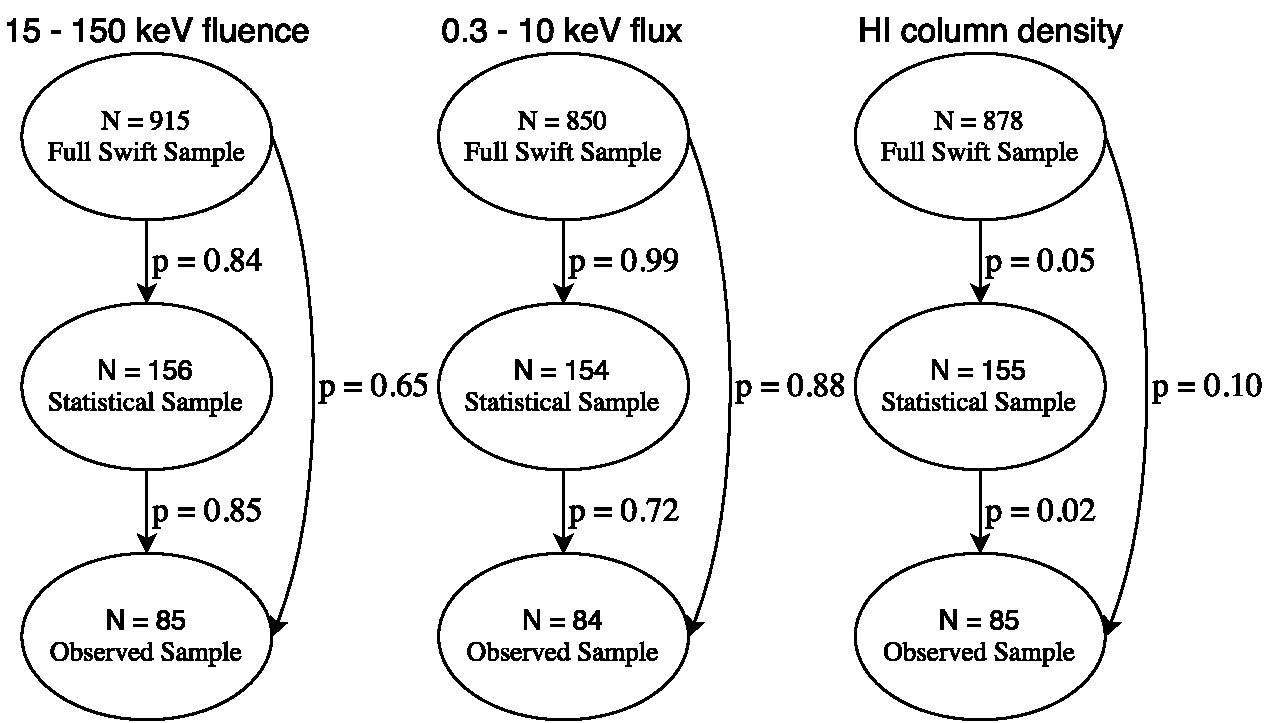
\includegraphics[width=9cm]{figures/XSGRB_p_values.pdf}}
	\caption{Relational graph shown the respective p-values that the different
	sample are drawn from the same underlying distribution. The arrows represent
	the comparison with each of the p-values are listed next to. Only in the HI
	column density distribution is there mild evidence against the null, but the
	discrepancy is mainly driven by a relatively larger fractional contribution
	from low-column hosts.}
	\label{fig:p_values}
\end{figure}

We therefore conclude that the sample presented here, to a high degree
represents the intrinsic properties of the GRBs in the full \textit{Swift} sample.
\todo{This doesn't quite feel exhaustive? Is there a better way of addressing the issue of completeness}

%%%%%%%%%%%%%%%%%%%%%%%%%%%%%%%%%%%%%%%%%%%%%%%%%%%%%%%%%%%%%%%%%%%%%%%%%%%%
\subsection{Properties of rejected triggers} \label{badbursts}
%%%%%%%%%%%%%%%%%%%%%%%%%%%%%%%%%%%%%%%%%%%%%%%%%%%%%%%%%%%%%%%%%%%%%%%%%%%%

GRB follow-up requires the immediate availability of the telescope in order to
successfully carry out spectroscopic observations. Out of the 158 \todo{Get
exact number} bursts in the statistical sample, 32($\sim$ 20 percent) \todo{Get
exact number} have not been observed due to conditions, not relating the GRB or
afterglow properties. The reasons includes unavailability of the telescope due
to technical maintenance such af mirror re-coating, a visitor rejecting the TOO
trigger, or bad weather at the observing site. Because this cut is irrespective
of the GRB properties, it is not expected that this should change sample
properties. Addressing whether this cut introduces a bias in the followed sample
is not trivial, but in terms of intrinsic GRB properties, the sample
distributions does not change significantly, as shown in Sect. \ref{completeness}.
\todo{Should this be quantified somehow?}

%%%%%%%%%%%%%%%%%%%%%%%%%%%%%%%%%%%%%%%%%%%%%%%%%%%%%%%%%%%%%%%%%%%%%%%%%%%%
\subsection{Sample darkness}
%%%%%%%%%%%%%%%%%%%%%%%%%%%%%%%%%%%%%%%%%%%%%%%%%%%%%%%%%%%%%%%%%%%%%%%%%%%%

A subset of all GRBs exhibit no detectable or very faint optical afterglow
\citep{Groot1998, Djorgovski2001, Fynbo2001}, which had been parametrized in
term of "darkness" \citep{Jakobsson2004, VanderHorst2009}. The X-ray properties
of this subset has previously been investigated \citep{DePasquale2003, Fynbo2009,
	Melandri2012}, finding a slightly higher X-ray luminosity compared to the
optically brights bursts combined with similar prompt characteristics pointing
towards a denser circumburst material. This indicates along with investigations
of host galaxy extinction \citep{Greiner2011, Kruhler2011, Hjorth2012}, that the
extinction of the optical afterglow is primarily driven by the presence of dust,
local to the burst \todo{Local dust reference}. Because the dust content of a
galaxy is correlated with the gas amount \citep{Bohlin1978, Guver2009}, we
expect the X-ray derived column densities for the bursts without an optical
afterglow to be higher than the ones without.

For all bursts with follow-up within 100 hours we can calculate the
"darkness"-parameter, $\beta_{OX}$ \citep{Jakobsson2004, Milvang-Jensen2012}. This required the
simultaneous measurement of the X-ray flux density and the optical flux density
which is in practice never possible. We use the measured acquisition camera
magnitude reported in Tab. \ref{tab:sample_overview} to get the optical flux
density at the beginning of the spectroscopic integration. Because we know the
delay between the follow-up and the \textit{Swift} trigger, we can use the
measured XRT burst lightcurve \citep{Evans2007,
	Evans2009}\footnote{http://www.swift.ac.uk/xrt\_curves/trigger\_numer/flux.qdp}
to infer the corresponding X-ray flux density. This is done by either linearly
interpolating between temporally neighboring XRT measurements of by
extrapolating the last few X-ray data points to the spectroscopic delay. When
the afterglow is not detected in the acquisition camera, an upper limit of $> 24$
mags is used, which propagates into an upper limit on $\beta_{OX}$.

In Fig. \ref{fig:betaOX} we compare the $\beta_{OX}$ - $N_H$ distribution with
the one presented in \citet{Fynbo2009}. We have replaced limits with values,
meaning that we artificially bias the distribution towards higher
$\beta_{OX}$-values because darker bursts naturally fainter in the optical
making the fraction of non-detections higher for lower $\beta_{OX}$. We
marginally confirm the result by \citet{Fynbo2009} that dark bursts $\beta_{OX}
< 0.5$) have slightly higher X-ray derived column densities, by calculating the
median, 14th, and 86th percentile of the distributions arising by separating the
sample at $\beta_{OX} = 0.5$. For bursts with $\beta_{OX} \geq 0.5$ we find
$\log(N_H) = 21.4_{-1.0}^{+0.7}$, whereas for $\beta_{OX} < 0.5$ we find
$21.8_{-0.9}^{+0.5}$, meaning that the median value for dark bursts is higher,
but with a great deal of overlap. A 2-sided KS test fails to reject the null
that they are drawn from the same distribution with $p = 0.43$, meaning there is
no clear evidence for a discrepancy.

\begin{figure}
	\centerline{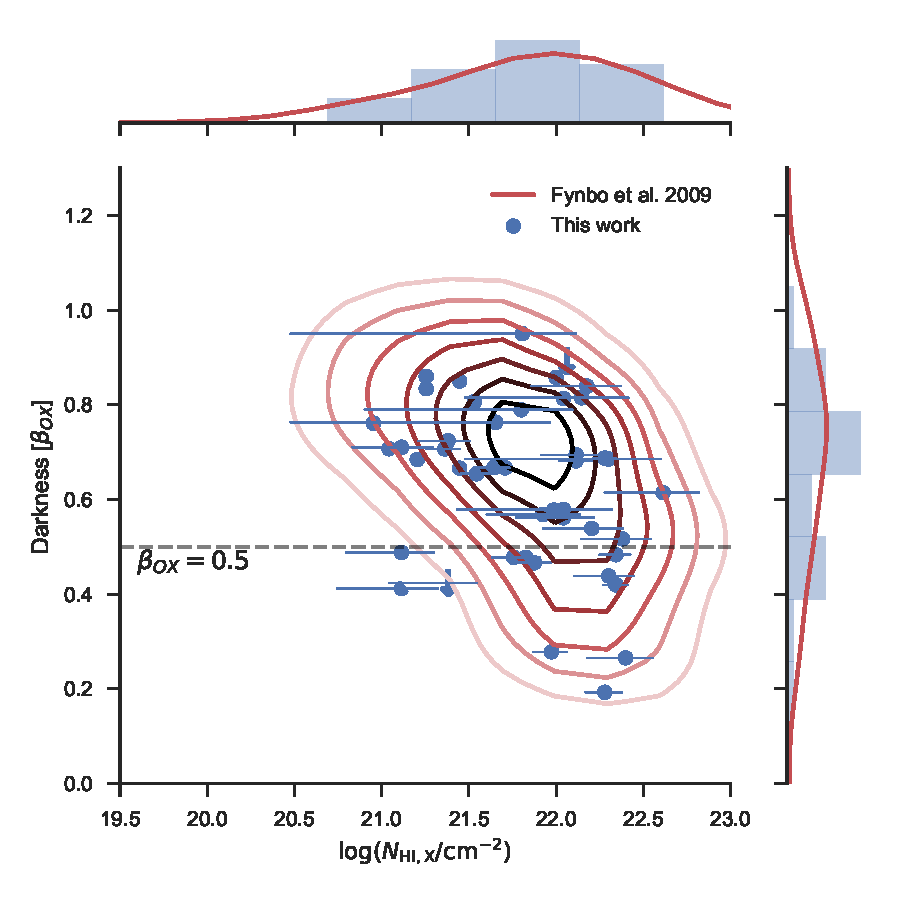
\includegraphics[width=9cm]{figures/betaOX.pdf}}
	\caption{Optical extinction relative to X-ray against X-ray derived hydrogen
	column densities. In red is shown the sample presented in \citet{Fynbo2009}
	where is lines indicate the kernel density estimate of the distribution where
	limits have been replaced with values. Darker colors represented denser points.
	The correcspoing marginal distributions are shown. In blue is the points for
	the bursts presented here along with the marginal histograms. Limits on
	$\beta_{OX}$ is shown by downwards facing arrows.}
	\label{fig:betaOX}
\end{figure}

Because we only follow up targets with either a clear afterglow or counterpart,
correctly associating a galaxy with a burst when there is no detected optical
afterglow is more difficult, see \citet{Levesque2010} and \citet{Perley2017} for
a recent example. Because the presence of optical transient is highly dependent
on the "darkness", we expect that the $\beta_{OX}$ sample is biased against dark
bursts. The larger relative fraction of upper limits for increased darkness is
visible both in the sample presented here and the one in \citet{Fynbo2009}. The
X-ray properties for the followed sample does not differ signicantly from the
statistical sample, as shown in Sect. \ref{completeness}. Using the table
maintained by Greiner\footnote{http://www.mpe.mpg.de/~jcg/grbgen.html} \todo{How
to reference this}, we can see how the presence of an optical afterglow affects
the follow-up statistics. 50.5 percent of all \textit{Swift}-detected bursts do
not have an detected optical afterglow, but this number also includes bursts
where no optical telescopes were available, so is a lower limit. For the bursts
entering our statistical sample, this number is $\sim$ 27 percent, close to the
maximum fraction of dark bursts \citep{Melandri2012}. Of the subsample (3) that
have actually been attempted, this number is $\sim$ 18 percent, confirming that
we are indeed biased against bursts with an optical afterglow in the
spectroscopic sample.

Since \textit{all} GRBs should have an optical afterglow, the presence of an optical afterglow is more a statement about the sensitivity than optical properties of the bursts. \todo{Hmm, how do I finish this?}


%%%%%%%%%%%%%%%%%%%%%%%%%%%%%%%%%%%%%%%%%%%%%%%%%%%%%%%%%%%%%%%%%%%%%%%%%%%%
\subsection{On the redshift distribution of GRBs}
%%%%%%%%%%%%%%%%%%%%%%%%%%%%%%%%%%%%%%%%%%%%%%%%%%%%%%%%%%%%%%%%%%%%%%%%%%%%

Because the redshift completeness of our statistical sample is just 54 percent
\todo{Get number}, making inference of the underlying redshift distribution of
GRBs on this ample is difficult. Because a large fraction of the bursts for which we were
unable to secure a redshift are missing due to terrestrial reasons, see Sect.
\ref{badbursts}, imposing additional unbiasing cuts on the sample can increase
the redshift completeness at the cost of sample size. As long as the cuts we
impose are not selective in terms of the burst properties, the sample properties
stay the same. The first cut we try is telescope availability such as bad
weather, visitor rejected the TOO, or unavailability of the instrument. Because
telescope availability is independent on the burst properties, by cutting away
these from our sample, the underlying redshift distribution should be conserved.
By trimming away the 30 bursts \todo{Get number} that can be rejected due to
telescope availability, the redshift completeness increases to 63 percent
\todo{Get number}. 

As is shown in Sect. \ref{timing}, the redshift completeness
decreases with increasing follow-up delay, we can additionally increase the
redshift completeness by imposing cuts on the follow-up delay. Our ability to
rapidly follow up a burst is also not dependent on the burst properties and
therefore we can additionally cut delays longer than 24 hours (all burst in the
sample are in principle observable within 24 hours). \todo{Unfinished section}


The biased introduced in the redshift distribution by the increased ability to
secure redshift of optically brighter bursts has been investigated by
\citet{Turpin2016} which find that we systematically find redshift for longer
GRBs. Additionally only the brightest GRBs are seen above redshift $z \gtrsim
1$. \todo{Unfinished section}




%%%%%%%%%%%%%%%%%%%%%%%%%%%%%%%%%%%%%%%%%%%%%%%%%%%%%%%%%%%%%%%%%%%%%%%%%%%%
\subsection{Hydrogen column densities}
%%%%%%%%%%%%%%%%%%%%%%%%%%%%%%%%%%%%%%%%%%%%%%%%%%%%%%%%%%%%%%%%%%%%%%%%%%%%

Because the locations of GRBs are associated with the most intensely starforming
regions \citep{Hogg1999, Bloom2002, Fruchter2006}, the GRB afterglow light has
to propagate through the large amounts of hydrogen fueling the star formation.
Because a significant fraction of the hydrogen has not been ionized yet, the
optical depth at the wavelength of \lya~is very high, saturating at the line
center. This causes a strong absorption system to appear in the afterglow
continuum. For bursts with $z \gtrsim 1.7$, the position of \lya~moves into the
spectroscopic coverage of X-shooter, meaning that we are able to detect this
absorption trough due to \lya.

Due of the stochastic nature of the \lya-forest, the blue wing of the Lyman
alpha absorption line is randomly superposed with forest systems, along with
strong absorption from \mnii~and \SIiii, making it notoriously difficult to
model. Additionally, Similarly so, the red wing has got the ISM signatures
imprinted on it, especially strong absorption due to \SIii, \sii~and \nv~which
can exhibit significant velocity structure. Along with instrumental effects, the
generative model for the data that we would use in a likelihood-based analysis
would be almost boundless in complexity, making formal fitting of the column
densities outside the scope of this paper.

Using an analytic approximation to an absorption line profile and it's
dependence on the column density \citep{TepperGarcia2006}, we overplot a
synthetic absorption line with a specified column density on our observed
spectrum. By tuning the value of the hydrogen column density until the synthetic
absorption line matches the spectrum, we can thereby infer the actual column
density of the GRB sight line in a manual way. In a similar fashion, the errors
on the hydrogen column can be inferred. We show the results of this procedure
for all bursts where possible in Fig. \ref{fig:HI1} and the inferred hydrogen
column densities in Tab. \ref{tab:HI}

\begin{table}[!ht]
\caption{Hydrogen column densities for all bursts exhibiting \lya~absorption in the spectral coverage of X-shooter. Corresponding fits are shown in Fig. \ref{fig:HI1}. \label{tab:HI}}
\centering
\begin{tabular}{cc}
\hline
\hline\noalign{\smallskip}
{GRB} & {Hydrogen Column} \\
\hline\noalign{\smallskip}

GRB~090809A & 21.7 $\pm$ 0.2    \\
GRB~090926A & 21.55 $\pm$ 0.10  \\
GRB~100219A & 21.20 $\pm$ 0.20  \\
GRB~100425A & 21.10 $\pm$ 0.20  \\
GRB~100728B & 21.2 $\pm$ 0.5  \\
GRB~110128A & 22.00 $\pm$ 0.15  \\
GRB~110818A & 21.9 $\pm$ 0.4    \\
GRB~111008A & 22.40 $\pm$ 0.10  \\
GRB~111107A & 21.0 $\pm$ 0.2    \\
GRB~120119A & 22.7 $\pm$ 0.2    \\
GRB~120327A & 22.0 $\pm$ 0.15   \\
GRB~120404A & 20.7 $\pm$ 0.3    \\
GRB~120712A & 19.95 $\pm$ 0.15  \\
GRB~120716A & 22.00 $\pm$ 0.15  \\
GRB~120815A & 22.05 $\pm$ 0.10  \\
GRB~120909A & 21.70 $\pm$ 0.10  \\
GRB~121024A & 21.85 $\pm$ 0.10  \\
GRB~121027A & 22.8 $\pm$ 0.3    \\
GRB~121201A\tablefootmark{a} & 22.0 $\pm$ 0.3  \\
GRB~121229A & 21.7 $\pm$ 0.2    \\
GRB~130408A & 21.8 $\pm$ 0.1    \\
GRB~130427B & 21.9 $\pm$ 0.3    \\
GRB~130606A & 19.91 $\pm$ 0.02  \\
GRB~130612A & 22.1 $\pm$ 0.2    \\
GRB~131011A & 22.0 $\pm$ 0.3    \\
GRB~131117A & 20.0 $\pm$ 0.3    \\
GRB~140311A & 22.40 $\pm$  0.15 \\
GRB~140430A & 21.8 $\pm$ 0.3    \\
GRB~140515A & 19.0 +- 0.5     \\
GRB~140614A & 21.6 $\pm$ 0.3    \\
GRB~141028A & 20.6 $\pm$ 0.15   \\
GRB~141109A & 22.1 $\pm$ 0.1    \\
GRB~150206A & 21.7 $\pm$ 0.4    \\
GRB~150403A & 21.8 $\pm$ 0.2    \\
GRB~150915A\tablefootmark{a} & 21.2 $\pm$ 0.3     \\
GRB~151021A & 22.2 $\pm$ 0.2    \\
GRB~151027B & 20.5 $\pm$ 0.2    \\
GRB~160203A & 21.75 $\pm$ 0.10  \\
GRB~160410A\tablefootmark{b} & 21.2 $\pm$ 0.2 \\
GRB~161014A & 21.4 $\pm$ 0.3    \\
GRB~161023A & 20.96 $\pm$ 0.05  \\



\hline\noalign{\smallskip}

\end{tabular}
\tablefoot{
\tablefoottext{a}{Has \lya~emission in the trough.}
\tablefoottext{b}{Short burst.}
} 
\end{table}

In a similar manner to how the X-ray derived column densities was used to assess
the sample completeness in Sect. \ref{completeness}, we addresses the same
question in terms of the optically derived hydrogen column densities. Using the
compilation by \citet{Tanvir2017} we have all 81 published HI values previously,
we can compare to the 39 new HI columns added by this sample. We note that this
sample increase the number of optically derived hydrogen column densities with
$\sim$ 50 percent. We compare the median, the 14th, and 86th percentiles of the
two distributions where the sample presented here has $21.8_{0.8}^{0.3}$ and the
rest of the litterature values has $21.5_{1.5}^{0.4}$. We see that the two
distribution has a large degree of overlap due to the large width of the
distributions, but find a slightly higher median value for the new sample
presented here. A 2-sided KS test gets us a p-value of p = 0.006, meaning
relatively large evidence against the null that the two samples are drawn from
the same underlying distribution. Because the bursts that have measurements of
the hydrogen column density are selected sole based on our ability to infer a
column, it is difficult to make any strong conclusions about the completeness in
terms of gas content. We show the comparison between the two samples in Fig.
\ref{fig:NH_dist}, where we additionally show the column-distribution for 12081
quasar DLAs published in \citet{Noterdaeme2012b}. The ability of the GRBs to
select the highest N$_H$ is immediately visible as is also noted previously
\citep{Prochaska2007, Fynbo2009}. The reason for this is the selection of sight
lines as random position of the QSO DLAs whereas the GRB forms in dense regions
in the host. The N$_H$ distribution has also be used the infer the position of
the gas in host \cite{Buchner2016} where a galaxy-wide gas reservoir is
preferred.

\begin{figure}
	\centering
	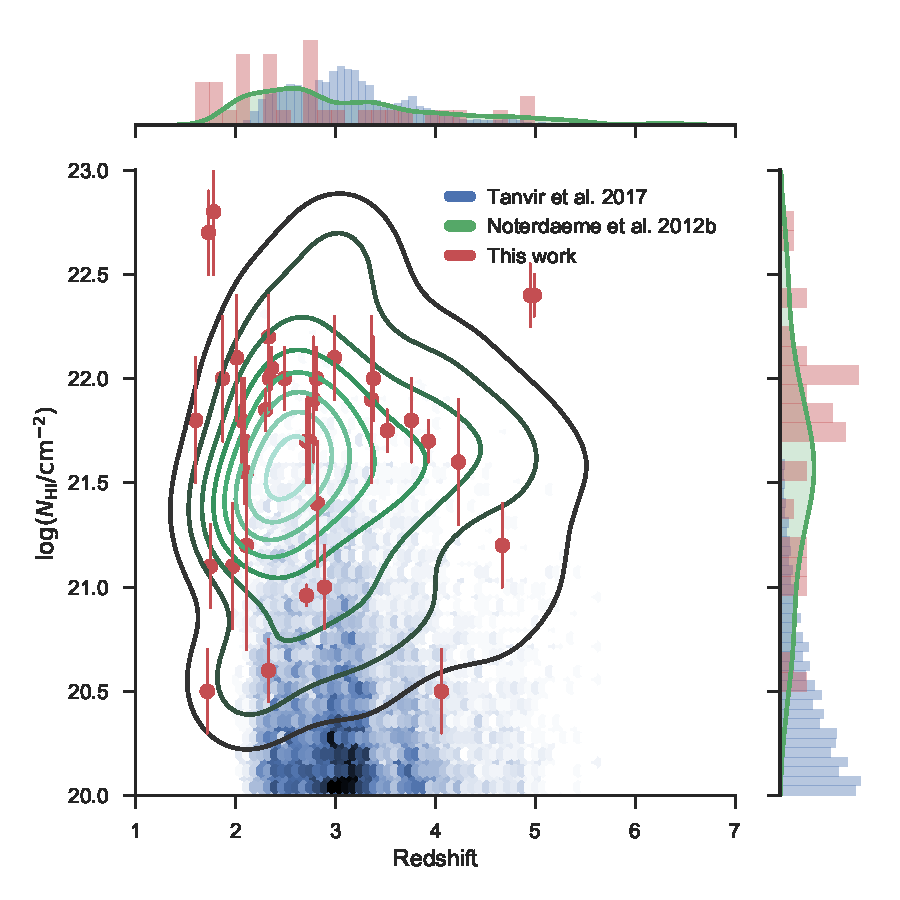
\includegraphics[width=9cm]{figures/NH_dist.pdf}
	\caption{Distributions of DLA hydrogen column densities for DLAs found in
		quasar absorption lines, from \citep{Noterdaeme2012b} in blue. Overplot in green is the kernel density estimate
		is the similar distribution, only for DLAs in GRB sightlines. Values are taken
		from the compilation in Tanvir2017 et al. (in prep)\citet{Tanvir2017}, along
		with the new values presented in this sample. The marginal distributions for
		the two distribution are also shown, where the different environments probed
		are clearly visible in the hydrogen column densities, as previously also noted
		in \citet{Fynbo2009}}
	\label{fig:NH_dist}
\end{figure}


%%%%%%%%%%%%%%%%%%%%%%%%%%%%%%%%%%%%%%%%%%%%%%%%%%%%%%%%%%%%%%%%%%%%%%%%%%%%
\section{Discussion and conclusions}
%%%%%%%%%%%%%%%%%%%%%%%%%%%%%%%%%%%%%%%%%%%%%%%%%%%%%%%%%%%%%%%%%%%%%%%%%%%%


In this paper we have presented the results
of a dedicated effort over the years 2009 -- 2016 to use the X-shooter 
spectrograph on the ESO-VLT to secure spectroscopic observations of 
afterglows and host galaxies of GRBs detected by {\it Swift}. This 
work was initiated by a consortium using Guaranteed Time on X-shooter, 
but over the years the project continuued in open time and the team was
opened to include any researchers interested in contribution to this 
effort.

The sample we present here include spectroscopic observations of 86 
systems fulfilling our sample criteria of which 72 are afterglow spectra 
and 14 are observations of the underlying host galaxies. 
UPDATE THIS.



%%%%%%%%%%%%%%%%%%%%%%%%%%%%%%%%%%%%%%%%%%%%%%%%%%%%%%%%%%%%%%%%%%%%%%%%%%%%
\section{Conclusion}
%%%%%%%%%%%%%%%%%%%%%%%%%%%%%%%%%%%%%%%%%%%%%%%%%%%%%%%%%%%%%%%%%%%%%%%%%%%%





\begin{acknowledgements}
JPUF, BMJ and DX acknowledge support from the ERC-StG grant EGGS-278202.  The
Dark Cosmology Centre is funded by the Danish National Research Foundation.  TK
acknowledges support by the European Commission under the Marie Curie
Intra-European Fellowship Programme in FP7.  AdUP acknowledges support by the
European Commission under the Marie Curie Career Integration Grant programme
(FP7-PEOPLE-2012-CIG 322307).  This work made use of data supplied by the UK
{\it Swift} Science Data Centre at the University of Leicester.  Finally, we
acknowledge expert support from the ESO staff at the Paranal and La Silla
observatories in obtaining these target of opportunity data.


This work made use of data supplied by the UK Swift Science Data Centre at the University of Leicester.
\end{acknowledgements}

\bibliographystyle{mnras}
\bibliography{XSGRB_sample}


\clearpage

\begin{figure*}[!h]
	\centering
	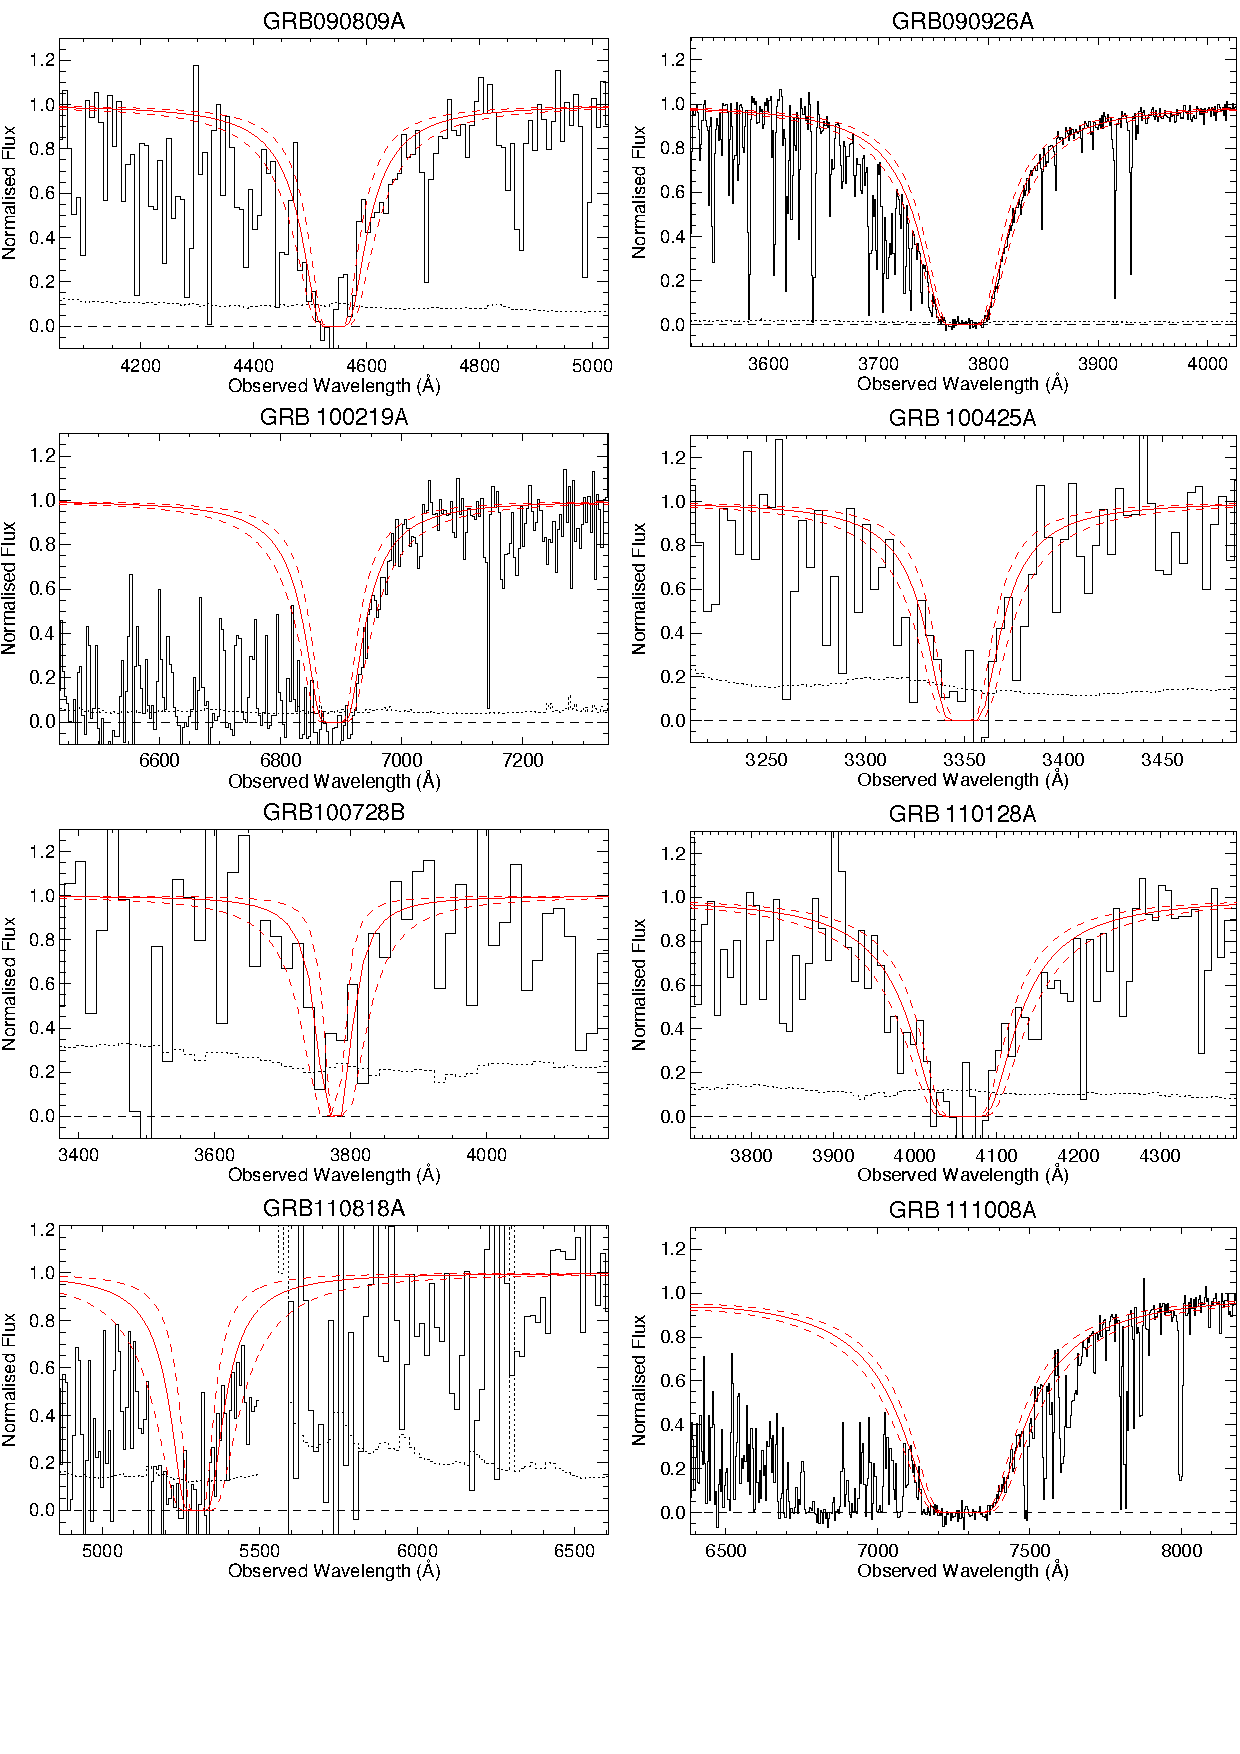
\includegraphics[page=1, width=16cm]{figures/HI_measurements.pdf}
	\caption{Measurements of the hydrogen column-densities for all bursts with a
		clear Lyman alpha absorption system. In solid black is shown the spectrum with
		black dotted giving the corresponding 1-$\sigma$ error. Black dashed shows zero
		flux density. The solid red line is the absorption of column density equal to
		the value presented in Tab. \ref{tab:HI} with the 1-$\sigma$ interval shown
		with dashed lines.}
	\label{fig:HI1}
\end{figure*}
\clearpage
\begin{figure*}[!h]
	\centering
	\includegraphics[page=2, width=16cm]{figures/HI_measurements.pdf}
	\caption*{Fig. \ref{fig:HI1}. continued.}
	\label{fig:HI2}
\end{figure*}
\clearpage
\begin{figure*}[!h]
	\centering
	\includegraphics[page=3, width=16cm]{figures/HI_measurements.pdf}
	\caption*{Fig. \ref{fig:HI1}. continued.}
	\label{fig:HI3}
\end{figure*}
\clearpage
\begin{figure*}[!h]
	\centering
	\includegraphics[page=4, width=16cm]{figures/HI_measurements.pdf}
	\caption*{Fig. \ref{fig:HI1}. continued.}
	\label{fig:HI4}
\end{figure*}
\clearpage
\begin{figure*}[!h]
	\centering
	\includegraphics[page=5, width=16cm]{figures/HI_measurements.pdf}
	\caption*{Fig. \ref{fig:HI1}. continued.}
	\label{fig:HI5}
\end{figure*}
\clearpage



\appendix


%%%%%%%%%%%%%%%%%%%%%%%%%%%%%%%%%%%%%%%%%%%%%%%%%%

\section{The complex error function and the Voigt profile} \label{voigt}
When modeling the spectral PSF, we need to evaluate the Voigt-profile. The Voigt profile, which is the convolution of the Gaussian and Lorentzian profiles, can, centered at zero, be written as \citep{pagnini2010} 
\begin{equation} 
\begin{split}
V(\lambda,\sigma, \gamma)  
& = G(\lambda, \sigma)  \otimes L(\lambda, \gamma) \\
& = \int_{-\infty}^{\infty} G(\xi, \sigma) L(\lambda - \xi, \gamma) d\xi \\
& = \int_{-\infty}^{\infty} \frac{1}{\sqrt{2 \pi} \sigma} e^{- \left( \frac{\xi}{\sqrt{2} \sigma}  \right)^2 } \frac{1}{\gamma \pi} \frac{\gamma^2}{(\lambda - \xi)^2 + \gamma^2} d\xi \\
& = \frac{\gamma}{\sqrt{2} \sigma} \frac{1}{ \pi^{3/2}}   \int_{-\infty}^{\infty} \frac{e^{- \left( \frac{\xi}{\sqrt{2} \sigma}  \right)^2 }}{(\lambda - \xi)^2 + \gamma^2}.
\end{split}
\end{equation}
We can by making the following substitution, $\xi = \sqrt{2} \sigma$ and $d\xi = \sqrt{2} \sigma dt$, write it as
\begin{equation} 
\begin{split}
V(\lambda,\sigma, \gamma)  
& =  \frac{\sqrt{2} \sigma}{ \sqrt{{\pi}}} \frac{\frac{\gamma}{\sqrt{2} \sigma}}{\pi}  \int_{-\infty}^{\infty} \frac{e^{- t^2 }}{(\lambda - \sqrt{2} \sigma t)^2 + \gamma^2} dt \\
& = \frac{1}{\sqrt{2 \pi} \sigma}  \frac{\frac{\gamma}{\sqrt{2} \sigma}}{\pi}  \int_{-\infty}^{\infty} \frac{e^{- t^2 }}{\left(\frac{\lambda}{\sqrt{2} \sigma} -  t\right)^2 + \left(\frac{\gamma}{\sqrt{2} \sigma}\right)^2} dt.	
\end{split}
\end{equation}
This form of the convolution is closely related to the complex probability function \citep{letchworth2007, abrarov2015a},
\begin{equation} 
\begin{split}
W(z)  
& = \frac{i}{\pi} \int_{-\infty}^{\infty} \frac{e^{-t^2}}{z - t}  
\end{split}
\end{equation}
for any complex argument, $z = x + iy$. The complex probability function can be expressed as a sum of a real an imaginary part \citep{benner1995, abrarov2015b},
\begin{equation} 
\begin{split}
W(x, y)  
& = K(x, y) + i L(x, y) \\
& = \frac{y}{\pi}  \int_{-\infty}^{\infty} \frac{e^{- t^2 }}{(x -  t)^2 +y^2} dt  + \frac{i}{\pi}  \int_{-\infty}^{\infty} \frac{(x - t)e^{- t^2 }}{(x -  t)^2 +y^2} dt,
\end{split}
\end{equation}
where is the real part, $\mathtt{Re}[W(x, y)] =  \sqrt{2 \pi} \sigma V(\lambda,\sigma, \gamma)$ if $x = \frac{\lambda}{\sqrt{2} \sigma}$ and $y = \frac{\gamma}{\sqrt{2} \sigma}$, which can be obtained by using the complex argument, $z = \frac{\lambda + i\gamma}{\sqrt{2} \sigma}$, in the complex probability function. If $\mathtt{Im}[z] \geq 0$, which is always guaranteed for the width of a spectral profile, the complex probability function equals the complex error function. The complex error function has numerous, fast, numerical approximations where in this work we use the \texttt{scipy.special.wofz} \citep{scipy} implementation.

%%%%%%%%%%%%%%%%%%%%%%%%%%%%%%%%%%%%%%%%%%%%%%%%%%

\section{Notes on Individual objects}

\subsection{GRB090313 (z = 3.373)}
The first GRB ever observed with X-shooter, during the commissioning of the
instrument, this data formed the basis of GCN
\#9015\footnote{\url{http://gcn.gsfc.nasa.gov/gcn3/9015.gcn3}} and is published
in \citet{DeUgartePostigo2010}. Due to the lingering brightness of GRB090313,
6.9 ks spectroscopic integration starting 45 hours after the BAT trigger reveals
a wealth of absorption features superposed on the afterglow continuum at a
common redshift of $z = 3.373$. Two intervening systems at $z = 1.959$ and $z =
1.800$ is identified based on strong \mgii-absorption. Because this burst is
observed before the instrument is science-verified, it does not enter into the
statistical sample.

\subsection{GRB090530 (z = 1.266)}
Observed during paranalization of the instrument, this data forms the basis of
GCN \#15571\footnote{\url{http://gcn.gsfc.nasa.gov/gcn3/15571.gcn3}}, but is not
published elsewhere. Observations began 20.6 hours after the BAT trigger and 4.8
ks spectroscopic integration in all three arms reveals the absorption signature
for a host at $z = 1.266$ from the detection of \mgii, \mgi, \SIii, \feii,
\aliii. Because this burst is observed before the instrument is
science-verified, it does not enter into the statistical sample.

\subsection{GRB090809 (z = 2.737)}
Observed during the first science verification period and was used for GCN
\#9761\footnote{\url{http://gcn.gsfc.nasa.gov/gcn3/9761.gcn3}} and is
additionally used as the basis for the master thesis by \'Asa Sk\'ulad\'ottir
(2010). 7.2 ks integration starting 10.2 hours after the GRB trigger notice
yields the clear afterglow continuum in all arms from with Lyman Limit located
in the beginning of the UVB coverage. The simultaneous detection of absorption
lines identified as \lya, \SIii, \oi, \SIi$^*$, \SIiv, \civ, \feii, \alii,
\aliii and \mgii at $z = 2.737$ sets it as the redshift of the GRB. Because this burst is observed before the instrument is
science-verified, it does not enter into the statistical sample.

\subsection{GRB090926 (z = 2.106)}
Starting during the second science verification period, this dataset forms the
basis of GCN \#9942\footnote{\url{http://gcn.gsfc.nasa.gov/gcn3/9942.gcn3}} and
is additionally published in \citet{DElia2010}. Spectroscopic integration
started 22 hours after the BAT trigger and from the acquistion camera the
optical afterglow has R = 17.9 mag (vega) at the beginning of the observations
which causes a very continuum to be seen in all arms. An absorption trough due
to \lya is clearly visible along with numerous metal resonance lines \civ,
\SIii, \SIii$^*$ \feii, \mgii, all at $z = 2.106$, marks this as the redshift of
the GRB. Because this burst is observed before the instrument is
science-verified, it does not enter into the statistical sample.

\subsection{GRB091018 (z = 0.971)}
The first burst observed during normal operation after science verification was
completed and there is the first burst that enter the statistical sample. This
data is the basis for GCN \#
10042\footnote{\url{http://gcn.gsfc.nasa.gov/gcn3/10042.gcn3}} and is published
in \citet{Wiersema2012}. With a bright afterglow and a rapid follow-up, this
spectrum is of pristine quality. The afterglow continuum is bright throughout
all spectroscopic arms which allows the ready detection of \alii, \aliii, \feii,
\mnii, \mgii, \mgi, and \caii al located at $z = 0.971$, setting is as the
redshift of the host.

\subsection{GRB091127 (z = 0.490)}
Obtained 4 days after the burst trigger, this data forms the basis for GCN \#
10233\footnote{\url{http://gcn.gsfc.nasa.gov/gcn3/10233.gcn3}} and is published
in \citet{Vergani2011}. Due to the late follow-up and a nearby moon, the S/N of
the afterglow continuum is poor especially in the UVB arm, why no clear
absorption lines are detected against the afterglow continuum, although see
\citet{Vergani2011} which report a tentative detection of \mgii. Emission lines
from the underlying host is clearly visible with lines from \oii, \hb, \oiii,
and \ha~all at $z = 0.490$. This bursts is additionally associated with
SN2009nz.

\subsection{GRB100205A  (z = na)}
Observed 3 days after the \textit{Swift} trigger. No afterglow or host detected
in 10.8 ks. GRB likely located at high
redshift\footnote{\url{http://gcn.gsfc.nasa.gov/gcn3/10399.gcn3}}. The spectrum
has not otherwise been published previously.

\subsection{GRB100219A (z = 4.667)}
The data presented here also formed the basis of GCN \#
10441\footnote{\url{http://gcn.gsfc.nasa.gov/gcn3/10441.gcn3}} and is published
in \citet{Thone2013}. Observations started 12.5 hours after the \textit{Swift}
trigger and has a total exposure time of 4.8 ks. Absorption features, including
those of \lya~and from a multitude of ions are detected against the afterglow
continuum at $z = 4.667$. Additionally, absorption from an intervening system
is found at $z = 2.181$.

\subsection{GRB100316B (z = 1.180)}
The data presented here also formed the basis of GCN \#
10495\footnote{\url{http://gcn.gsfc.nasa.gov/gcn3/10495.gcn3}}. The spectrum
has not otherwise been published previously. Observations started 44 minutes
after the \textit{Swift} trigger and has a total exposure time of 2.4 ks.
Absorption features from \feii, \alii, \aliii,	\mgii~and \mgi~are well detected
against the afterglow continuum at $z = 1.180$. Additionally, strong absorption
lines from \feii~and \mgii~from an intervening system are found at $z = 1.063$.

\subsection{GRB100316D (z = 0.059)}
The data presented here also formed the basis of GCN \#
10512\footnote{\url{http://gcn.gsfc.nasa.gov/gcn3/10512.gcn3}}, GCN \#
10513\footnote{\url{http://gcn.gsfc.nasa.gov/gcn3/10513.gcn3}}, GCN \#
10543\footnote{\url{http://gcn.gsfc.nasa.gov/gcn3/10543.gcn3}} and is published
in \citet{Bufano2012} and \citet{Starling2011}. This GRB is very close by and
has an associated SN, SN2010bh, and has therefore undergone intense follow-up. The data
presented here consists of a subset of the entire VLT/X-shooter campaign,
covering the four first observing days while the afterglow still contributes
significantly to the total emission. The first observations started 10 hours
after the burst, before the SN was discovered, and targeted the star-forming
'A'-region\citep{Starling2011}, not the GRB. A very rich spectrum containing a
multitude of emission lines puts the host at $z = 0.059$. For three consequtive
nights, 58, 79 and 101 hours after the \textit{Swift} trigger, the afterglow
was observed as it transitioned into the spectrum of a high-velocity Ic-BL SN.
The observations taken 79 and 101 hours after the burst are taken under
programme 084.D-0265(A) (PI: Benetti), but with an identical setup to the first
two observations.

\subsection{GRB100418A (z=0.624)}
The data presented here also formed the basis of GCN \#
10620\footnote{\url{http://gcn.gsfc.nasa.gov/gcn3/10620.gcn3}} and GCN \#
10631\footnote{\url{http://gcn.gsfc.nasa.gov/gcn3/10631.gcn3}} and is published
in \citet{DeUgartePostigo2011}. The burst have been followed up in three epochs
of observations, 0.4, 1.4, and 2.4 days after the burst, each lasting 4.8 ks.
The unambiguous redshift of the host, $z=0.624$, is found from the simultaneous
detection of emission features belonging to nebular lines, including \hi, \oii,
\oiii, \neiii, \nii, \sii, \siii, and \hei~as well as absorption features due
to the presence of \znii, \crii, \feii, \mnii, \mgii, \mgi, \tiii, and \caii,
all at a consistent redshift. Temporal evolution of the fine structure lines
belonging to \feii$^*$ is found between the epochs.

\subsection{GRB100424A (z=2.465)}
The data presented here also formed the basis of GCN \#
14291\footnote{\url{http://gcn.gsfc.nasa.gov/gcn3/14291.gcn3}}. The spectrum
has not otherwise been published previously. Observations carried out, long
after the burst has faded.  Emission lines from the host are detected at
$z=2.465$.

\subsection{GRB100425A (z=1.1755)}
The data presented here also formed the basis of GCN \#
10684\footnote{\url{http://gcn.gsfc.nasa.gov/gcn3/10684.gcn3}} and is used in
Skuladottir (2010), but not published elsewhere. Observations started 4
hours after the \textit{Swift} trigger, totaling 2.4 ks. Absorption features
from \mgii~and \feii~in the afterglow continuum are detected at $z=1.1755$.

\subsection{GRB100615A (z=1.398)}
The data presented here also formed the basis of GCN \#
14264\footnote{\url{http://gcn.gsfc.nasa.gov/gcn3/14264.gcn3}}, but not
published elsewhere. Host observation of a dark burst\citep{DElia2011} taken
long after the afterglow has faded. Emission lines from the host belonging to
\oii, \neiii, \oiii~and \ha~are detected at a common redshift of $z=1.398$.

\subsection{GRB100621A (z=0.542)}
The data presented here also formed the basis of GCN \#
10876\footnote{\url{http://gcn.gsfc.nasa.gov/gcn3/10876.gcn3}}, but not
published elsewhere. Beginning 7.1 hours after the GRB, 2.4 ks observations
reveal emission lines from \oii, \hb~and \oiii~at a common redshift of
$z=0.542$ and a very weak afterglow continuum.

\subsection{GRB100625A (z=0.452)}
The data presented here is of the candidate host galaxy, taken long after the
burst has faded and have not previously been published. 4.8 ks of exposure
reveals a weak continuum present in all arms, but an absence of emission lines.
This could indicate that the host primarily contains a older stellar
population. The redshift, $z=0.452$, is taken from \citet{Fong2013}.


\subsection{GRB100724A* (z = 1.288)}
The data presented here also formed the basis of GCN \#
10971\footnote{\url{http://gcn.gsfc.nasa.gov/gcn3/10971.gcn3}}. The spectrum
has not otherwise been published previously. The observations were carried out
in RRM starting 11 min after the GRB trigger. See section \ref{RRM}, for a
description of the RRM scheme. Absorption lines from several ionic species are
detected in the afterglow continuum at a common redshift of $z = 1.288$. This
is not a part of the statistical sample.

\subsection{GRB100728B (z=2.106)}
The data presented here also formed the basis of GCN \#
11317\footnote{\url{http://gcn.gsfc.nasa.gov/gcn3/11317.gcn3}}. The spectrum
has not otherwise been published previously. Starting 22 hours after the burst
trigger, 7.2 ks of observations reveals a faint afterglow continuum with \lya-
and \mgii-absorption at $z=2.106$. Due to a malfunctioning ADC, the sensitivity
of X-shooter is depressed with respect to normal operations, resulting in a
poorer throughout. Additionally, the position of the trace on the slit moves
due to atmospheric differential refraction.

\subsection{GRB100814A (z=1.439)}
The spectra presented here has not been published previously. The
observations consists of three visits, the first beginning only 0.9 hours
after the \textit{Swift} trigger, the other two visits were 2.13 and 98.40
hours after the trigger, respectively. A bright afterglow continuum is
present in all visits, allowing identification of absorption features
belonging to a wide range of ions at $z=1.439$. A complex velocity structure
in the absorption features belonging to \mgii, shows several components,
separated by as much as 500km/s, pointing to a likely merger scenario in
the host.

\subsection{GRB100816A (z=0.805)}
The data presented here also formed the basis of GCN \#
11123\footnote{\url{http://gcn.gsfc.nasa.gov/gcn3/11123.gcn3}}. The spectrum
has not otherwise been published previously. This short GRB was observed 28.4
hours after the GRB trigger. 4 x 1200 s of exposure reveals two distinct sets
of emission lines, spatially offset $\lesssim 1 \arcsec $, very close in
redshift space, $z=0.8034$ and $z=0.8049$, indicating either an interacting
host or some complex velocity structure of the host. Faint underlying continua
are present under both sets of lines.

\subsection{GRB100901A (z=1.408)}
The data presented here has been published in \citet{Hartoog2013}. Because of
the unusual lingering brightness of this GRB, 2.4s of observations taken 65.98
hours after the GRB trigger still reveals an afterglow continuum visible across
the entire spectral coverage of X-shooter. Absorption lines from a wide range
ion put the redshift at $z=1.408$, with intervening absorption systems at $z =
1.3147$ and $z = 1.3179$.

\subsection{GRB101219A (z=0.718)}
This data has not been published before. Starting 3.7 hours after the GRB
trigger, 7.2 ks of exposure time reveals a very faint continuum in the visual
and near-infrared, only visible when heavily binning the images. No redshift
estimate is available from these observations.  Late-time Gemini-North
observations reveal emission lines from the host at
$z=0.718$\footnote{\url{http://gcn.gsfc.nasa.gov/gcn3/11518.gcn3}}.

\subsection{GRB101219B (z=0.552)}
The data presented here also formed the basis of GCN \#
11579\footnote{\url{http://gcn.gsfc.nasa.gov/gcn3/11579.gcn3}} and is published
in \citet{Sparre2011}.	The first observation, taken 11.6 hours after the burst
trigger and lasting 4.8ks, reveals absorption from \mgii~and \mgi~in the host
located at $z = 0.552$ on a featureless continuum visible across the entire
coverage of X-shooter.  Subsequent observations taken 16 and 37 days after the
trigger shows the fading spectral signature of a SN, SN2010ma.


\subsection{GRB110128A (z=2.339)}

\subsection{GRB110407A (z=na)}

\subsection{GRB110709B (z=2.1092 (NEW!!!!))}
This is a late-time observation (> 1 year) and has previously been used in
\citet{Perley2016a}. In this reduction of the 7.2 ks spectroscopic integration,
the tentative detection of \oiii~reported in \citet{Perley2016a} is confirmed
along with low-significance detection of \ha~at the end of the spectral
coverage, both at a consistent redshift, $z=2.1092$, securing it as the redshift
of the GRB.


\subsection{GRB110715A (z=0.82)}

\subsection{GRB110721A (z=0.382)}

\subsection{GRB110808A (z=1.348)}

\subsection{GRB110818A (z=3.36)}

\subsection{GRB111005A (z=0.013)}

\subsection{GRB111008A  (z=4.989)}

\subsection{GRB111107A (z=2.893)}

\subsection{GRB111117A (z=2.211)}

\subsection{GRB111123A  (z=3.151)}

\subsection{GRB111129A (z=na)}

\subsection{GRB111209A (z=0.677)}

\subsection{GRB111211A (z=0.478)}

\subsection{GRB111228A (z=0.716)}




\subsection{GRB120118B (z = 2.943)}
The data presented here also formed the basis of GCN \#
14225\footnote{\url{http://gcn.gsfc.nasa.gov/gcn3/14225.gcn3}}, but is not
published otherwise. This late-time observation of the host of GRB120118B
consists of 3.6 ks exposures and contains emission lines belonging to \oii and
\oiii at $z =	2.943$, suggested to be redshift of the host.

\subsection{GRB120119A (z = 1.728)}
The data presented here has not been published before. Three epochs of
observations have been obtained, the first two immediately after the burst, and
the last one long after the afterglow had faded. Starting 1.4 hours after the
\textit{Swift} trigger, the first epoch contains bright afterglow continuum.
Rich in absorption features belonging to a multitude of ions, $z =	1.728$ is
estimated for the host with intervening systems at $z =	1.476$, $z = 1.214$, $z
= 0.662$ and $z = 0.632$. The second epoch, obtained 4.5 hours after the burst
contains the fading afterglow. A third epoch is obtained $>1$ year after the
GRB in which emission lines from \hb~and \ha~are found at the redshift of the
host, confirming the association of the absorption line system and the host.

\subsection{GRB120211A (z = 2.346)}
The data presented here has been published in \citet{Kruhler2015}. Two
observations of the host of GRB120211A has been obtained, starting 2013.02.17,
$> 1 year$ after the burst has faded. A redshift for this object has been
reported by \citet{Kruhler2015} and the features seen by those authors are
reproduced in these reductions, confirming $z =	2.346$.

\subsection{GRB120224A (z = 1.10 NEW!!!)}
The data presented here has formed the basis of GCN \#
12991\footnote{\url{http://gcn.gsfc.nasa.gov/gcn3/12991.gcn3}}, and has also
been published in \citet{Kruhler2015}. Starting 19.8 hours after the GRB
trigger, a total exposure time of 2.4 ks reveals a faint continuum, starting at
$\sim$ 7000 \AA~and extending all the way through 25000 \AA. We detect a $\sim
2 \sigma$ emission line which, if interpreted as \ha, gives $z = 1.10$,
supporting the redshift reported by \citet{Kruhler2015}.

\subsection{GRB120311 (z = 0.350 NEW!!!)}
The data presented here has formed the basis of GCN \#
12991\footnote{\url{http://gcn.gsfc.nasa.gov/gcn3/12991.gcn3}}, but is not
published otherwise. Starting just before twilight, 3.65 hours after the burst,
a faint afterglow continuum is detected at all wavelengths. Due to the
faintness of the afterglow, no absorption features are discernible superposed
on the continuum. Displaced from the afterglow continuum by 1\farc4, emission
lines belonging to \hb, \oiii~and \ha~are detected at $z = 0.350$. The line
belonging to \ha~shows some extended emission toward the afterglow continuum.
The angular distance between the two sources correspond to a projected distance
in the host plane of 6 kpc, posing a potential problem for the host redshift,
unless the GRB ocurred in a merging system. The extended emission in \ha,
supports this interpretation. This burst is not apart of the statistical sample.

\subsection{GRB120327A (z = 2.813)}
The data presented here also formed the basis of GCN \#
13134\footnote{\url{http://gcn.gsfc.nasa.gov/gcn3/13134.gcn3}} and is published
in \citet{DElia2014}. The observation consists of two visits, 2.13 hrs and
29.98 hrs after the burst, with an afteglow continuum visible in all arms for
both visits. We detect absorption features from Ly-limit, \lya, \cii/\cii$^*$,
\SIii/\SIii$^*$, \ali, \feii ~and \mgii ~are detected at a consistent redshift,
$z = 2.813$.

\subsection{GRB120404A (z = 2.876)}
The data presented here has formed the basis of GCN \#
13227\footnote{\url{http://gcn.gsfc.nasa.gov/gcn3/13227.gcn3}}, but is not
published otherwise. 9.6 ks integration, starting 15.7 hours after the
\textit{Swift}-trigger reveals a low-intensity afterglow continuum on which
absorption from \lya is detected in two distinct regions at redshifts $z=2.876$
and $z=.255$. These absorption systems are confirmed by ionic absorption
features at both of these redshifts.


\subsection{GRB120422A (z = 0.283)}
The data presented here also formed the basis of GCN \#
13257\footnote{\url{http://gcn.gsfc.nasa.gov/gcn3/13257.gcn3}} and is published
in \citet{Schulze2014}. A GRB-SN, this burst has been followed up multiple
times. The data presented here only contain the first epoch in which the
afterglow is still visible and before the rise of SN2012bz. Starting 16.5 hours
after the burst, 4.8 ks integration time captures both the host and the burst
in emission. A blue afterglow continuum is detected at all wavelengths covered
by X-shooter, on which \mgii absorption at $z = 0.283$ is found. Offset by
1\farc75, the host is clearly detected at a consistent redshift with a rich
emission line spectrum, the lines extending towards to burst.

\subsection{GRB120712A (z = 4.175)}
The data presented here also formed the basis of GCN \#
13460\footnote{\url{http://gcn.gsfc.nasa.gov/gcn3/13460.gcn3}} and is not
published elsewhere. 4.8 ks integration time, starting 10.5 hours after the BAT
trigger, shows a bright afterglow continuum starting at $\sim$ 4720 \AA,
signifying the onset of the Lyman alpha forest, for a GRB located at $z =
4.175$. Absorption features from \lya, \feii, \mgii~and \SIii~are readily
detected at a consistent redshift.

\subsection{GRB120714B (z = 0.398)}
The data presented here also formed the basis of GCN \#
13477\footnote{\url{http://gcn.gsfc.nasa.gov/gcn3/13477.gcn3}}, but is not
published elsewhere. Observations of this burst started 7.8 hours after the GRB
trigger, lasting 4.8 ks. A continuum is visible across the entire spectral
coverage of X-shooter, with both emission lines from  \oii, \hb, \oiii~and \ha,
as well as absorption from \mgii~detected at $z = 0.398$, securely setting it
as the redshift of the GRB.


\subsection{GRB120716A (z = 2.486)}
The data presented here also formed the basis of GCN \#
13494\footnote{\url{http://gcn.gsfc.nasa.gov/gcn3/13494.gcn3}}, but is not
published elsewhere. Despite observations starting 62 hours after the
\textit{Swift} trigger and lasting 3.6 ks, a bright afterglow is clearly seen,
along with a plethora of absorption features. Absorption of \lya-photons in the
host leaves a broad trough, from which the Lyman alpha forest is visible
bluewards, all the way down to the Lyman limit. Metal absorption lines from
\cii, \SIii, \oi, \feii, \civ, \SIiv, including fine structure transitions
identified as \cii$^*$, \SIii$^*$, \feii$^*$ and metastable \NIii~lines are all
detected at $z = 2.486$


\subsection{GRB120722A (z = 0.959)}
The data presented here also formed the basis of GCN \#
13507\footnote{\url{http://gcn.gsfc.nasa.gov/gcn3/13507.gcn3}}, but is not
published elsewhere. On 4.8 ks integration time, starting 10 hours after the
burst trigger, the simultaneous detection of absorption features belonging to
\mgii~and \feii~superposed on a blue continuum, and emission lines from \oii,
\hg, \hb, \oiii~and \ha, all at $z = 0.959$, confidently sets it as the
redshift of the GRB.



\subsection{GRB120805A (z $\sim$ 3.9 NEW!!!)}
A separate reduction of this burst has been published in \citet{Kruhler2015},
but not otherwise. Starting 9 days after the burst trigger, this is host
observation and does not contain any afterglow continuum. In 3.6 ks integration
time, we detect a faint continuum visible from 4500 \AA~and all the way through
21000 \AA, in contrast to what is found previously. The continuum from 4500 -
6000 \AA is detected at very low significance. If the drop at 4500 \AA~is the
Lyman limit, this fits with Lyman alpha at $\sim$ 6000 \AA, giving $z \sim
3.9$. The absence of nebular lines if due to \oii~falling in a telluric
absorption band and the rest being shifted out of the wavelength coverage.

\subsection{GRB120815A* (z = 2.358)} 
Not a part of the statistical sample, thisburst also formed the basis of  GCN
\# 13649\footnote{\url{http://gcn.gsfc.nasa.gov/gcn3/13649.gcn3}} and is
published in \citet{Kruhler2013}. Observations started 1.69 hours after the BAT
trigger and consist of 2.4 ks integration. A bright afterglow continuum is
detected across the entire spectral coverage of X-shooter, with a multitude of
absorption lines superposed. Absorption features from the host at $z = 2.358$
include a DLA as well as metal absorption lines from \nv, \sii, \SIii, \oi,
\civ, \SIiv, \feii, \alii, \aliii, \mnii, \mgii, and \mgi. Additionally
fine structure lines from \NIii and \feii are exited local to the GRB.
Intervening systems are found at $z = 1.539$, $z = 1.693$, and $z = 2.00$.


\subsection{GRB120909A (z = 3.929)}
The data presented here has formed the basis of GCN \#
13730\footnote{\url{http://gcn.gsfc.nasa.gov/gcn3/13730.gcn3}}, but is not
published otherwise. A very rapid follow-up, starting only 1.7 hours after the
BAT trigger, this 1.2 ks observation captures a very bright afterglow
continuum, starting at 4500 \AA, signifying the onset of the Lyman limit for a 
system at $z = 3.929$. Absorption from high-column density hydrogen leaves very
prominent absorption features in the form of \lya, \lyb, and \lyg, visible in
the Lyman alpha forest. Metal absorption lines arising from \feii, \NIii,
\SIii, \sii, \alii, \aliii, \cii, \oi, \civ, and \znii~are all detected along
with the corresponding fine structure lines from (\feii$^*$, \SIii$^*$,
\oi$^*$, \oi$^**$, \cii$^*$), securely anchoring the redshift of the host.




\subsection{GRB120923A (z = $\gtrsim8$?)}






\subsection{GRB121024A (z = 2.300)}
The data presented here also formed the basis of GCN \#
13890\footnote{\url{http://gcn.gsfc.nasa.gov/gcn3/13890.gcn3}} and is published
in \citet{Friis2015}. Also rapid, starting 1.8 hours after the \textit{Swift}
trigger, a bright afterglow continuum is visible across all arms. A broad
absorption feature from Lyman alpha, along with narrow lines from \civ, \SIii,
\SIiv, \feii, \sii, and \alii, as well as fine structure lines associated with
\SIii$^*$ are all detected at $z = 2.300$, securely setting it as the redshift
of the GRB.

\subsection{GRB121027A (z = 1.773)}		
The data presented here has formed the basis of GCN \#
13930\footnote{\url{http://gcn.gsfc.nasa.gov/gcn3/13930.gcn3}}, but is not
published otherwise. Starting 69.6 hours after the GRB trigger, that we detect
the afterglow continuum a so high significance in all arms with 8.4 ks
integration, testifies to the brightness of this burst. The concurrent
identification of emission lines from \oiii~and absorption from \civ, \alii,
\aliii, \mgi, \mgii, and \feii, tightly constrains the redshift of the burst to
be $(z = 1.773$




\subsection{GRB121201A (z = 3.385)}		




\subsection{GRB121229A (z = 2.707)}		





\subsection{GRB130131B (z = 2.539)}		





\subsection{GRB130408A (z = 3.758)}
The data presented here also formed the basis of GCN \#
14365\footnote{\url{http://gcn.gsfc.nasa.gov/gcn3/14365.gcn3}}. The spectrum
has not otherwise been published previously. The observations consists of two
600sec spectra taken 1.9hrs after the burst. We detect absorption features from
a wide range of ions. We also detect intervening absorption at $z=1.255$ and
$z=3.248$.



\subsection{GRB130418A (z = 1.218)}	




\subsection{GRB130427A (z = 0.34)}	




\subsection{GRB130427B (z = 2.78)}	




\subsection{GRB130603B (z = 0.356)}	





\subsection{GRB130606A (z = 5.913)}
The data presented here also formed the basis of GCN \#
14816\footnote{\url{http://gcn.gsfc.nasa.gov/gcn3/14816.gcn3}} and is published
in \citet{Hartoog2015}. The observations consists of three 2x600sec visits
starting 7.1 hrs after the burst at fairly high airmass. We detect absorption
features from a wide range of ions at $z=5.913$ as well as intervening
absorption at $z=2.3103, 2.5207, 3.4515, 4.4660, 4.5309, 4.5427, 4.6497 $ and $
4.7244$.




\subsection{GRB130612A (z = 2.006)}	





\subsection{GRB130615A (z = $~3$?)}	





\subsection{GRB130701A (z = 1.155)}	





\subsection{GRB131011A (z = 1.874)}	





\subsection{GRB131030A (z = 1.296)}	





\subsection{GRB131103A (z = 0.599)}	




\subsection{GRB131105A (z = 1.686)}	




\subsection{GRB131117A (z = 4.042)}	




\subsection{GRB131231A (z =0.642)}	



\subsection{GRB140114A (z = $\sim2.8$?)}	



\subsection{GRB140213A (z = 1.208)}	



\subsection{GRB140301A (z = 1.416)}	



\subsection{GRB140311A (z = 4.95)}	



\subsection{GRB140430A (z = 1.601)}	



\subsection{GRB140506A  (z = 0.889)}	



\subsection{GRB140515A (z = $\sim6.32$?)}	



\subsection{GRB140614A (z = 4.233)}	



\subsection{GRB140622A (z = 0.959)}	



\subsection{GRB141028A (z = 2.332)}	



\subsection{GRB141031A  (z = na)}	



\subsection{GRB141109A (z = 2.993)}	



\subsection{GRB150206A (z = 2.087)}	



\subsection{GRB150301B (z = 1.517)}	



\subsection{GRB150403A (z = 2.06)}	



\subsection{GRB150423A (z = 1.394)}	



\subsection{GRB150428A (z = na)}	



\subsection{GRB150514A (z = 0.807)}	



\subsection{GRB150518A (z = 0.256)}	



\subsection{GRB150616A (z = 1.188)}	



\subsection{GRB150727A (z = 0.313)}	



\subsection{GRB150821A (z = 0.755)}	



\subsection{GRB150831A (z = na)}	



\subsection{GRB150910A (z = 1.359)}	



\subsection{GRB150915A (z = 1.968)}	



\subsection{GRB151021A (z = 2.330)}
The data presented here also formed the basis of GCN \#
18426\footnote{\url{http://gcn.gsfc.nasa.gov/gcn3/18982.gcn3}} and is not
published elsewhere. The observation was carried out in RRM starting 44 minutes
after the GRB trigger. We detect absorption features from a wide range of ions
at $z=2.330$ as well as intervening absorption at $z=1.49$.



\subsection{GRB151027B (z = 4.063)}	



\subsection{GRB151029A (z = 1.423)}	



\subsection{GRB151031A (z = 1.167)}	



\subsection{GRB160117B (z = 0.87)}	



\subsection{GRB160203A (z = 3.517)}
The data presented here also formed the basis of GCN \#
18982\footnote{\url{http://gcn.gsfc.nasa.gov/gcn3/18982.gcn3}} and is not
published elsewhere. The observation was carried out in RRM starting 18 minutes
after the GRB trigger. We detect absorption features from a wide range of ions
at $z=3.517$ as well as intervening absorption at $z=2.203$.

\subsection{GRB160228A (z = 1.64)}	



\subsection{GRB160303A (z = na)}	



\subsection{GRB160314A (z = 0.726)}	



\subsection{GRB160410A (z = 1.717)}	



\subsection{GRB160425A (z = 0.555)}	



\subsection{GRB160625B (z = 1.406)}	



\subsection{GRB160804A (z = 0.736)}
The data presented here also formed the basis of GCN \#
19773\footnote{\url{http://gcn.gsfc.nasa.gov/gcn3/19773.gcn3}}, but is not
published elsewhere. Observations started 22.37 hours after the BAT trigger and
lasted for 2.4ks. The afterglow continuum is detected across the entire
spectral coverage of X-shooter and absorption lines from \mgi, \mgii, \feii~and
\alii~are found at $z = 0.736$. At the same redshift, emission lines from \oii,
\oiii, \ha, \hb, \hg, \nii, \sii, \siii~are found. A second epoch, lasting
3.6ks, is obtained after the afterglow has faded, confirming the emission line
detections.


\subsection{GRB161001A (z = 0.891?)}	



\subsection{GRB161007A (z =4.6 ??? NEW!!!)}
This data has not been published elsewhere. Observations for GRB161007A started
323 hours after the burst trigger and contains the potential host. 4 x 600 seconds
of observations reveals a faint continuum rising abruptly above the noise at
$\sim$ 6850 \AA~and continuing through 21000 \AA. A very low significance
continuum is detected at shorter wavelengths, down to $\sim$ 6000 \AA. If the
host is located at $z \sim 4.6$, the drop in continuum flux is the Lyman alpha
break and the absence of nebular emission lines is due to \oii being shifted
out of the wavelength coverage. Alternatively, an early-type host at $z = 0.71$
could exhibit the 4000 \AA break at 6000 \AA, but due to the preference of
long-duration GRBs for star-forming galaxies, this is the least likely
explanation, why we believe the high-z solution.

\subsection{GRB161014A (z =2.823)}
The data presented here also formed the basis of GCN \#
20061\footnote{\url{http://gcn.gsfc.nasa.gov/gcn3/20061.gcn3}}, but is not
published elsewhere. Starting 11.6 hours after the GRB trigger, 4.8 ks of
integration time captures the afterglow continuum across all three
spectroscopic arms. A broad absorption trough due to Lyman alpha is visible,
along with metal absorption features from \mgii, \SIii, \cii, \civ, \alii,
\aliii, and	\feii, all at $z =2.823$. Similar to GRB140506 \citep{Fynbo2014}, a
break in the continuum shape is detected bluewards of 6000\AA, possible
signifying some anomalous form of extinction.


\subsection{GRB161023A (z = 2.710)}	


\subsection{GRB161117A (z = 1.549)}	


\end{document}


